\documentclass{beamer}
\mode<presentation>
{
  \usetheme{Madrid}      % or try Darmstadt, Madrid, Warsaw, ...
  \usecolortheme{dolphin} % or try albatross, beaver, crane, ...
  \usefonttheme{default}  % or try serif, structurebold, ...
  \setbeamertemplate{navigation symbols}{}
  \setbeamertemplate{caption}[numbered]
} 

\usepackage[english]{babel}
\usepackage[utf8]{inputenc}
\usepackage[T1]{fontenc}
\usepackage{pdfpages}


\title[Wikidata WikiProject COVID-19]{Wikidata WikiProject COVID-19}
\author[User:TiagoLubiana]{Tiago Lubiana - University of São Paulo}
\date[25/06/2020]{June 25th, 2020}


\begin{document}



{
\setbeamercolor{background canvas}{bg=}

\includepdf[pages=1]{fig/first_slide.pdf}
}



\begin{frame}
  \titlepage
\end{frame}

% Uncomment these lines for an automatically generated outline.
%\begin{frame}{Outline}
%  \tableofcontents
%\end{frame}


\section{Intro}

\begin{frame}{Wikipedia \& COVID-19}

\begin{itemize}
    \item Wikipedia is a major source of information about COVID-19

\end{itemize}

\begin{figure}
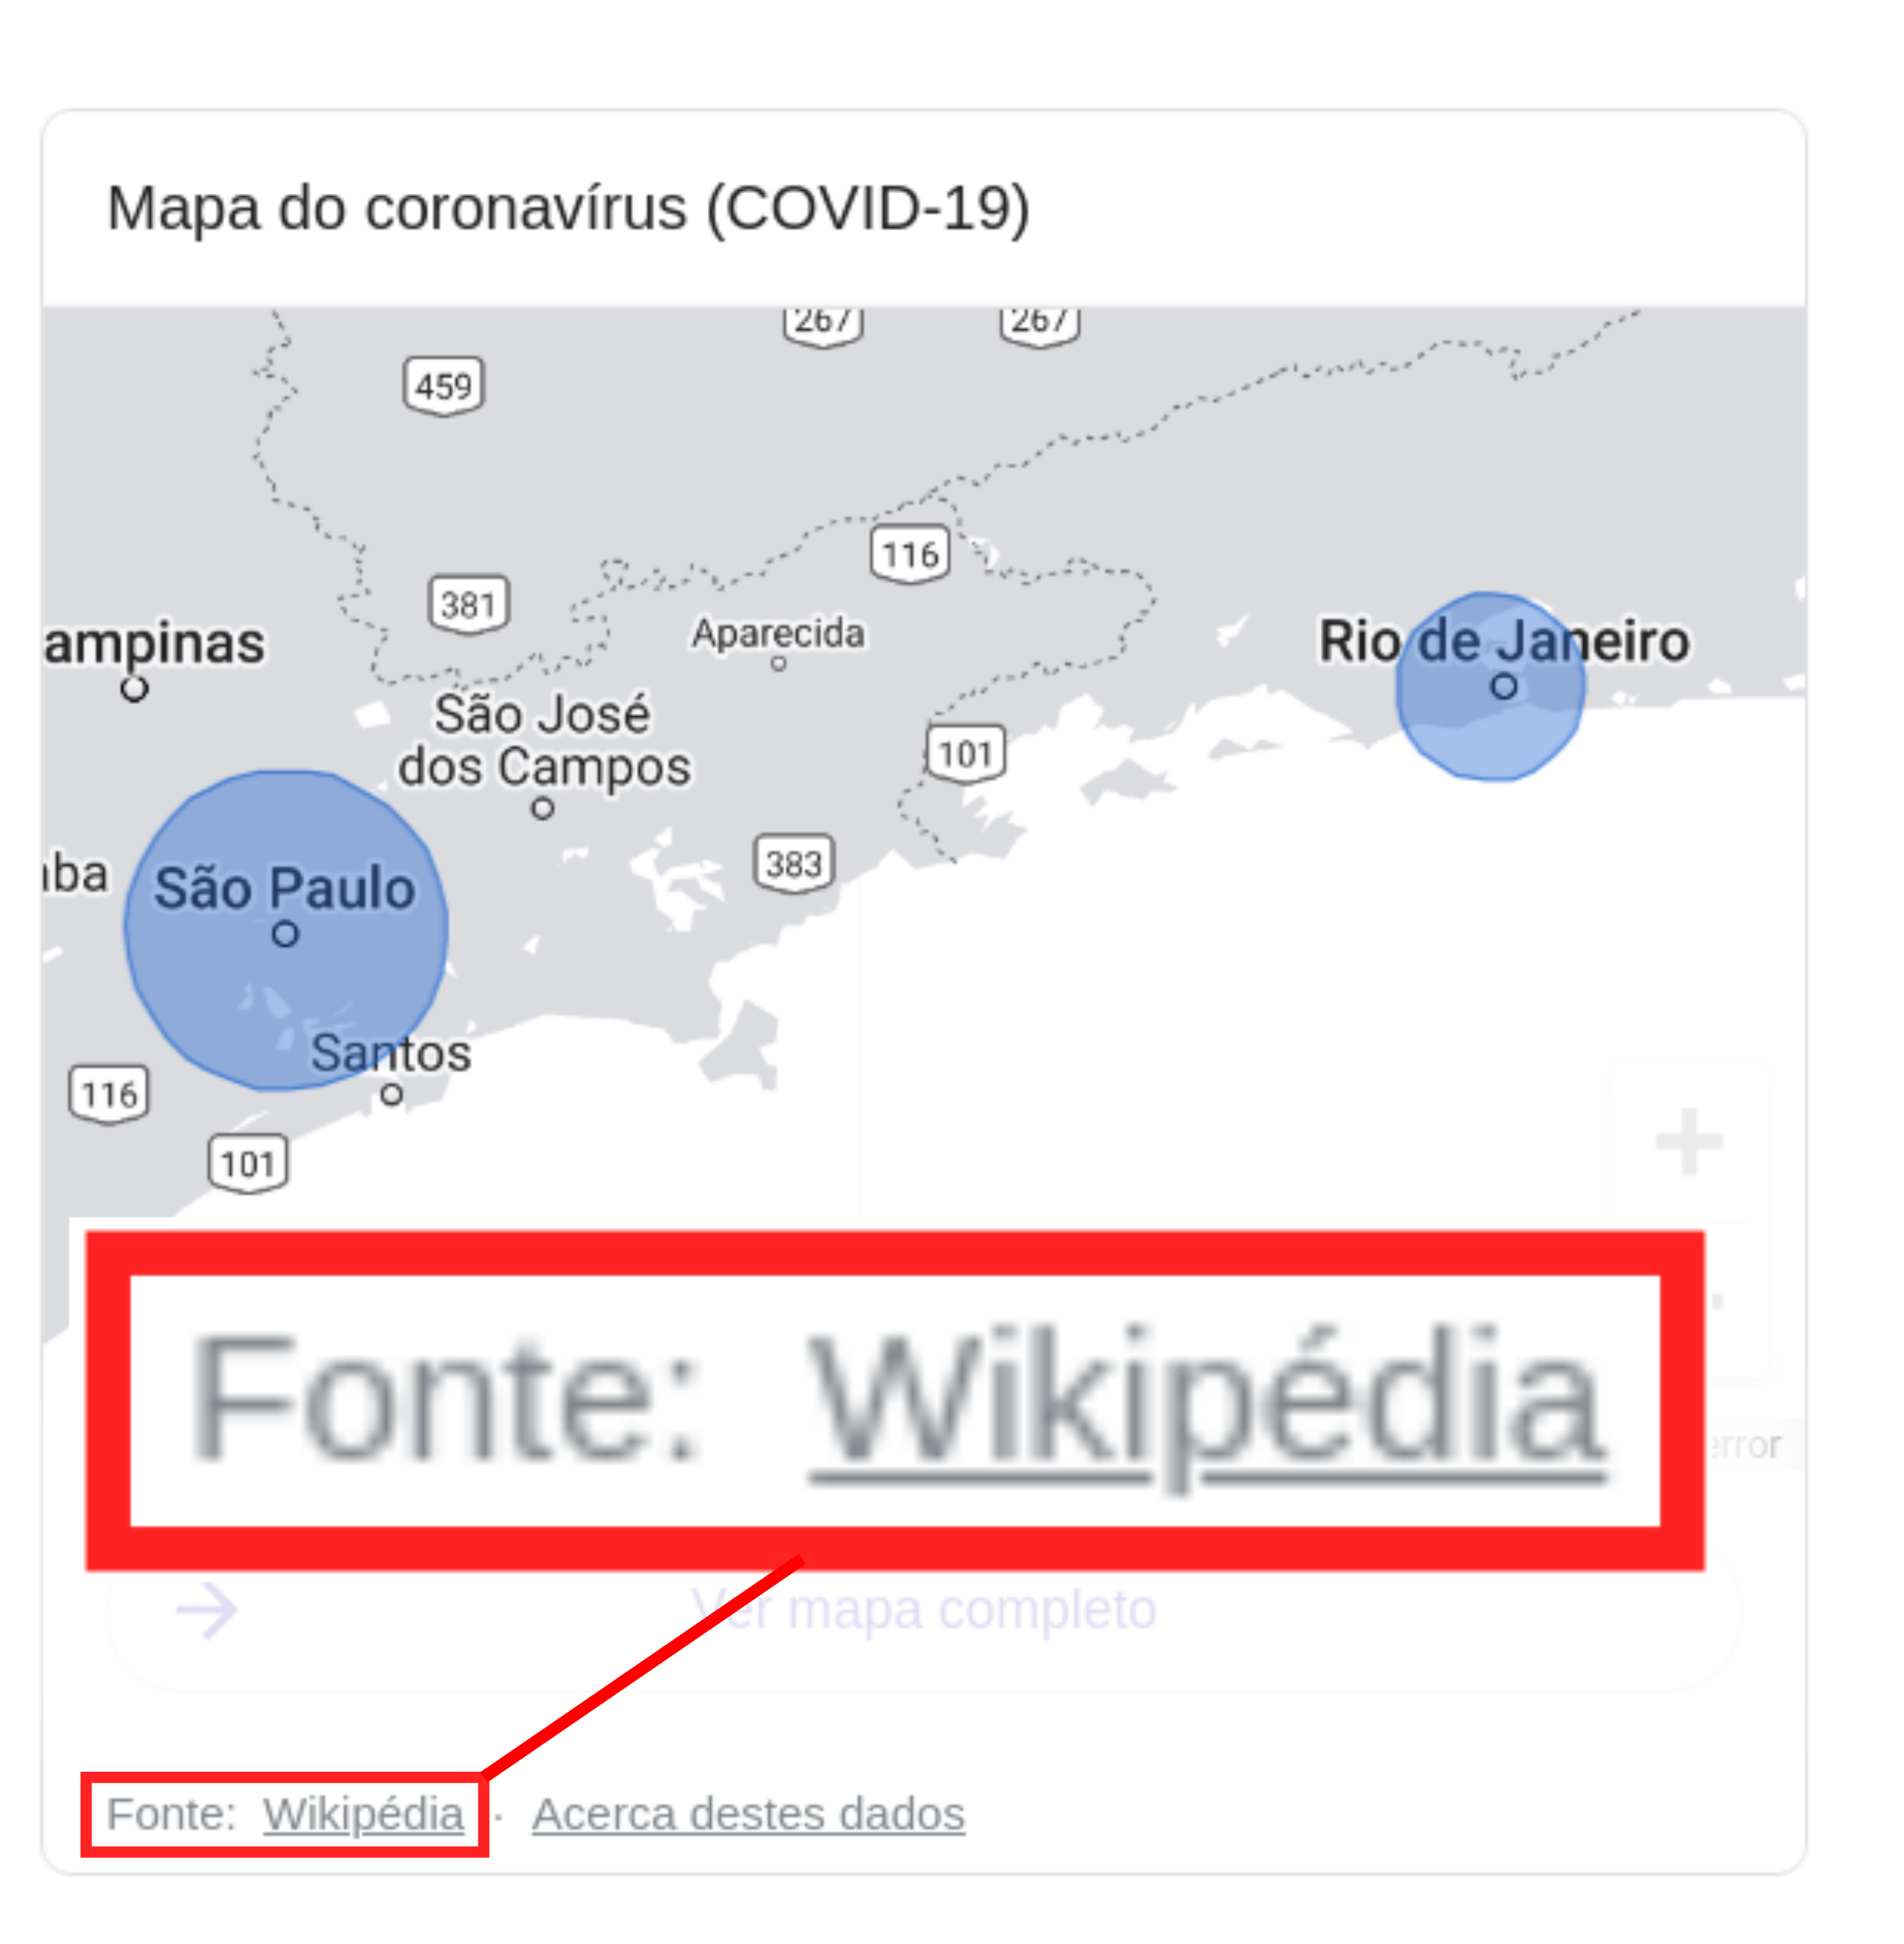
\includegraphics[scale=0.45]{fig/wikipedia_in_google.png}
\end{figure}

 https://wikimediafoundation.org/covid19/data/
 
\end{frame}



\begin{frame}{Wikipedia \& COVID-19}

\begin{itemize}
    \item Wikipedia is a major source of information about COVID-19
    
    \begin{itemize}
        \item https://wikimediafoundation.org/covid19/data/
    \end{itemize}
    
\end{itemize}

\begin{figure}
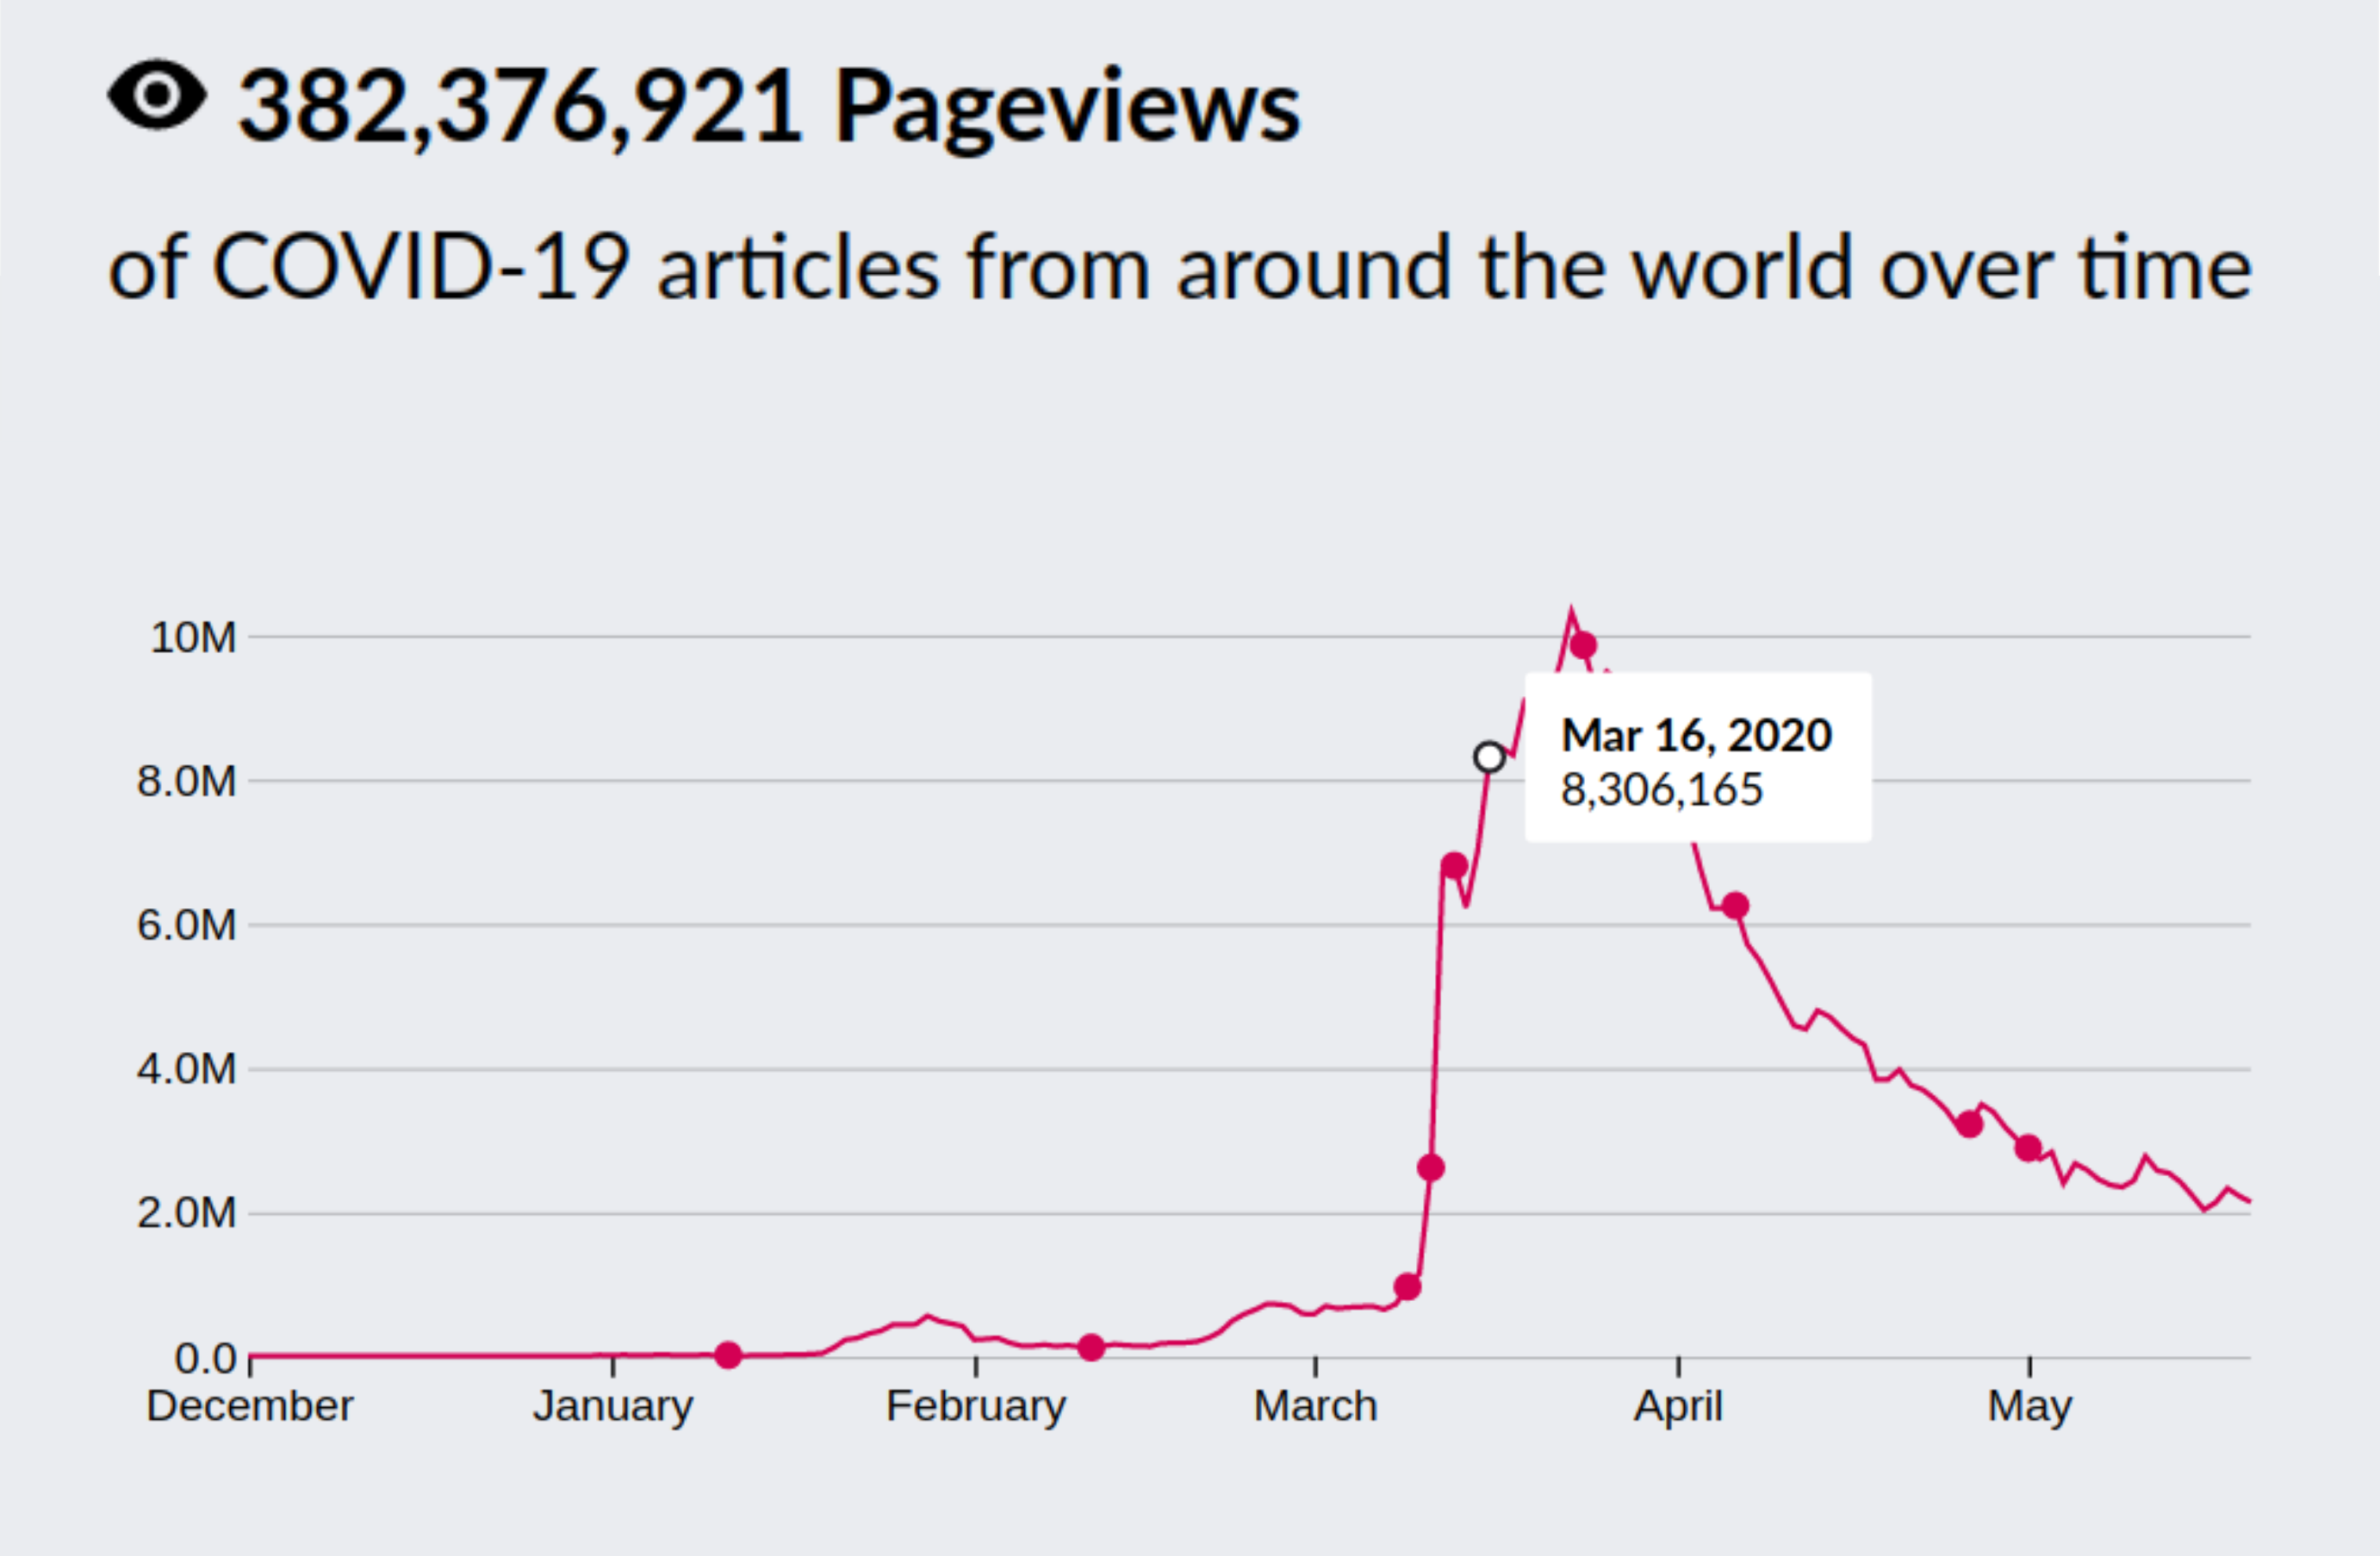
\includegraphics[scale=0.45]{fig/wikipedia_access_covid_19.png}
\end{figure}
\end{frame}


\begin{frame}{Wikidata is there to organize Wikipedia's data}

\begin{figure}
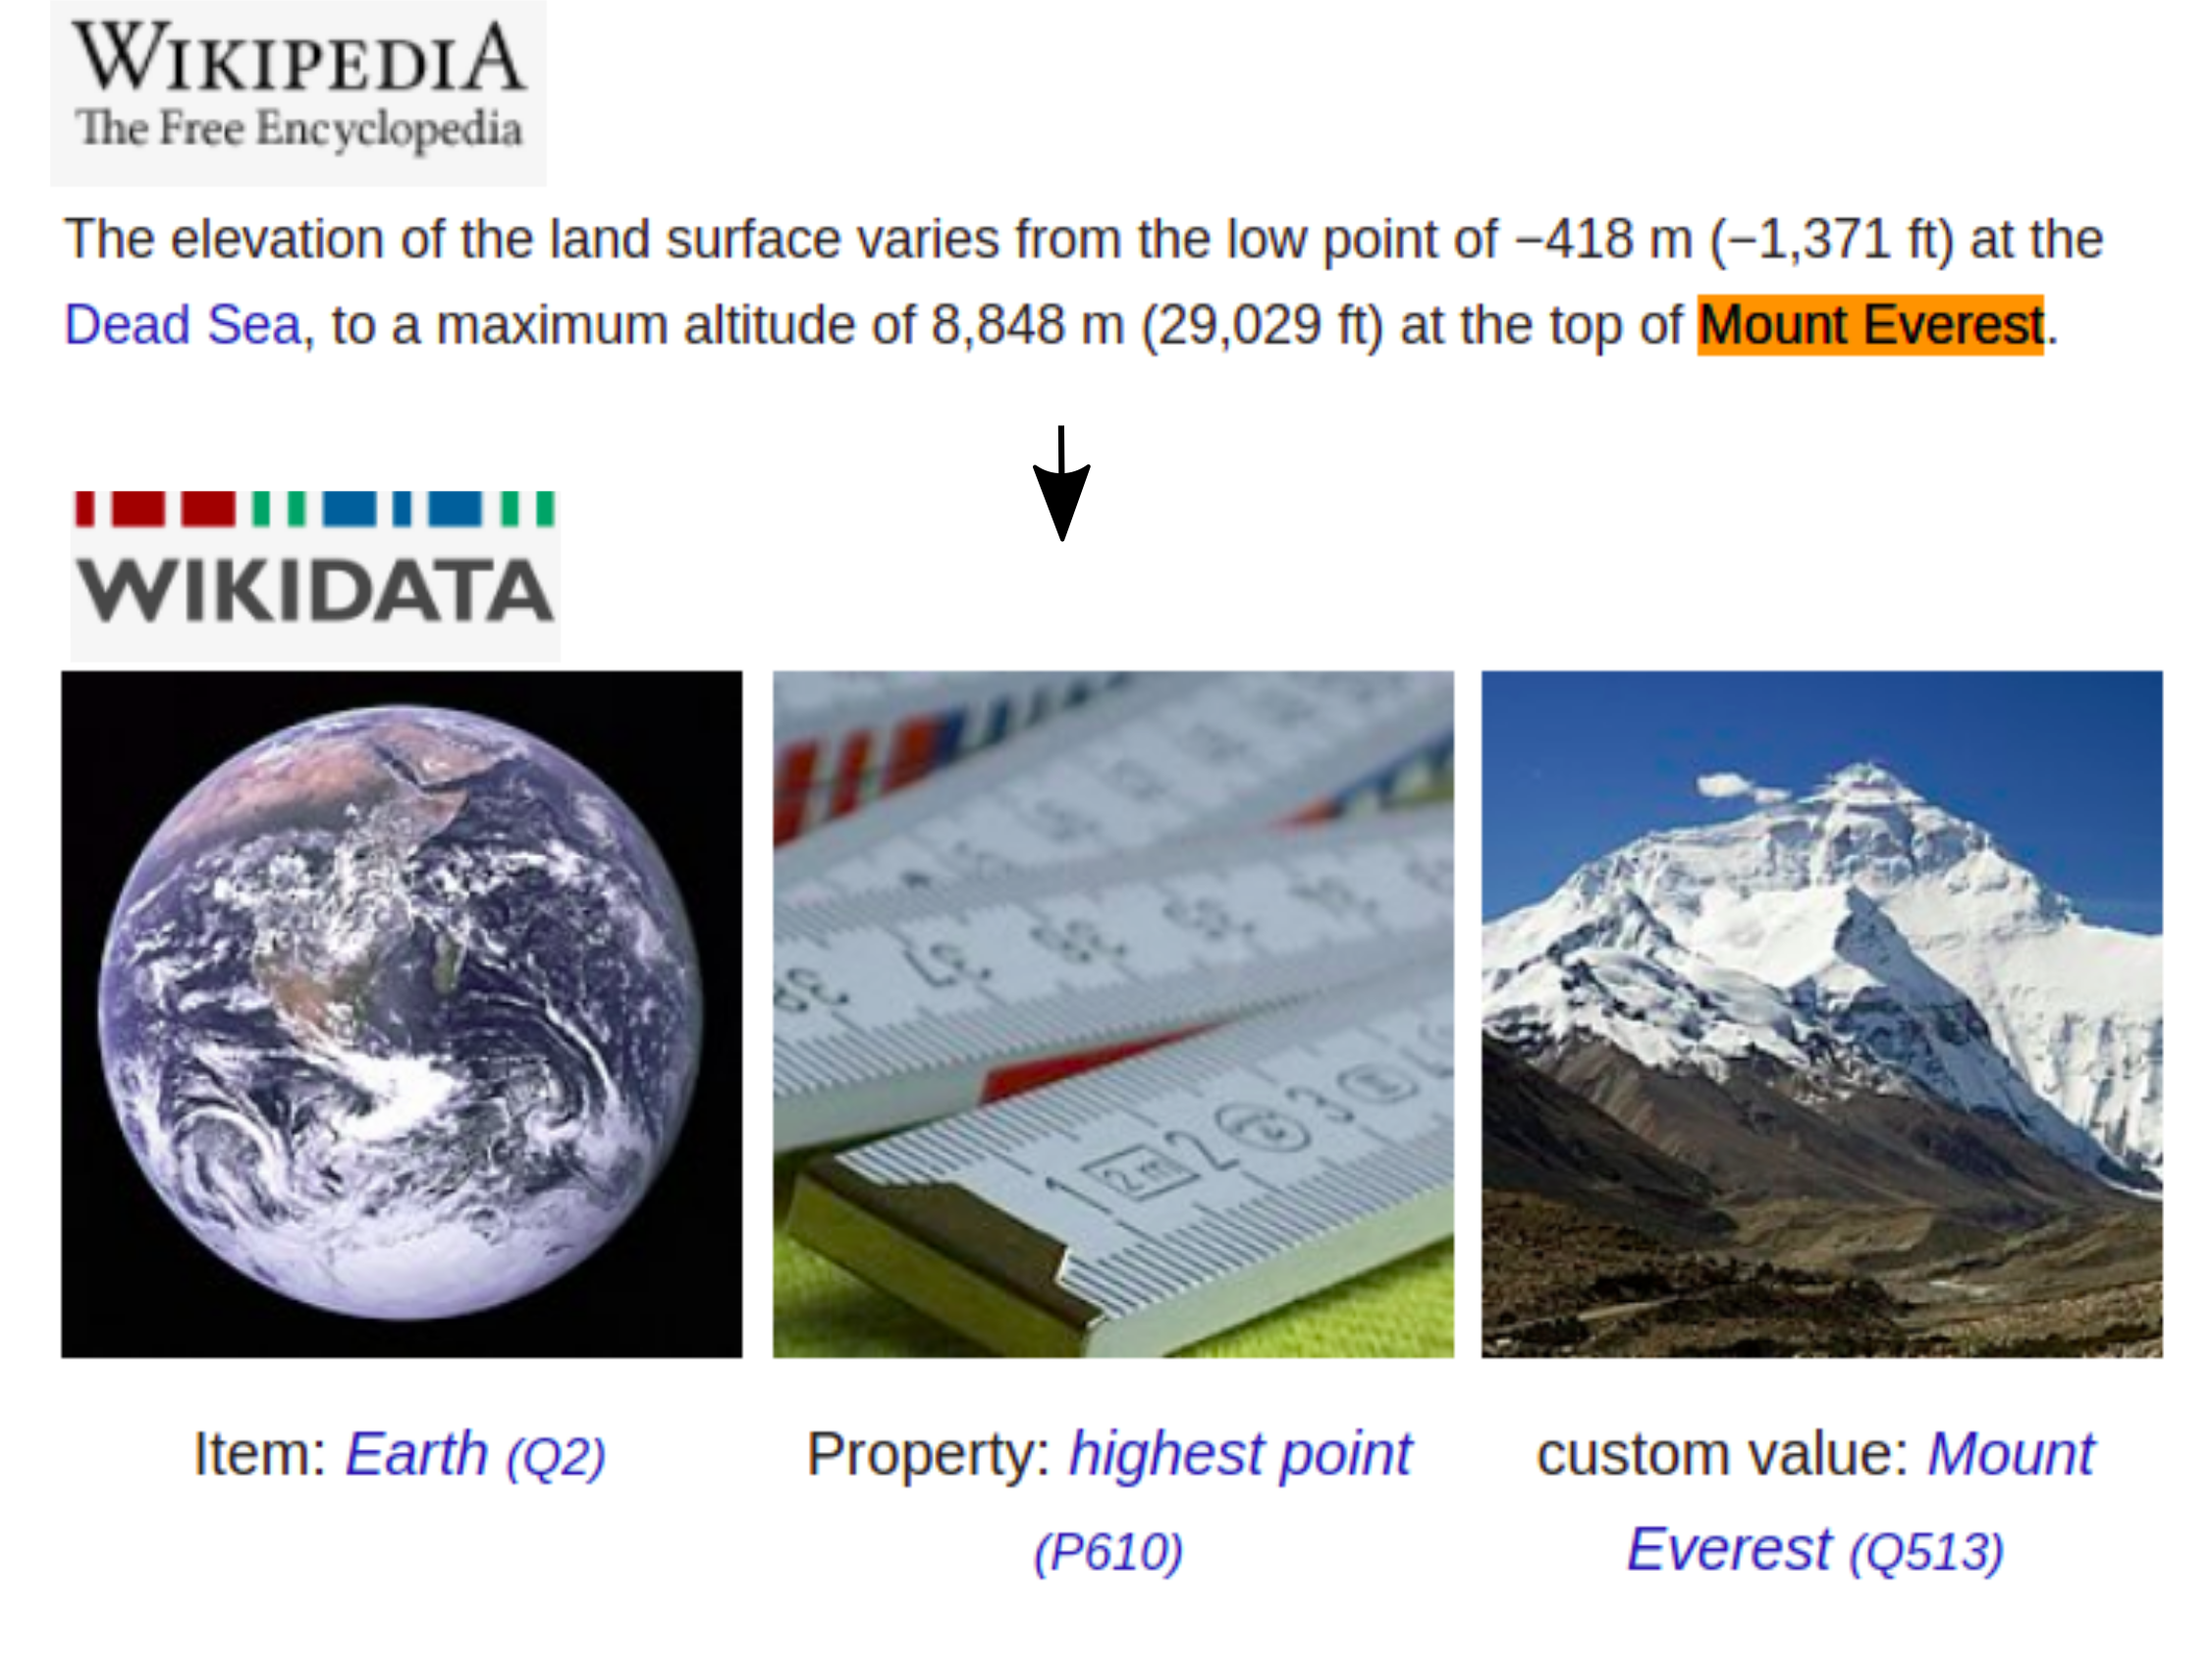
\includegraphics[scale=0.45]{fig/intro wikidata.png}
\end{figure}

\end{frame}






%         Data quality monitoring and data modeling for a quickly evolving situation
%        "Oiling the machine" for future crises
%        Standardization of data accross Wikipedias. 
%        Providing structured data for secondary visualizations



\begin{frame}{Wikidata's way of organizing information}

\begin{itemize}
    \item Wikidata's structure is similar to a RDF triplestore
\end{itemize}
\begin{figure}

\includegraphics[scale=0.7]{fig/item_property_value.png}
\end{figure}

\end{frame}


\begin{frame}{Wikidata is an improvement on Wikipedia raw table storage}

\begin{figure}
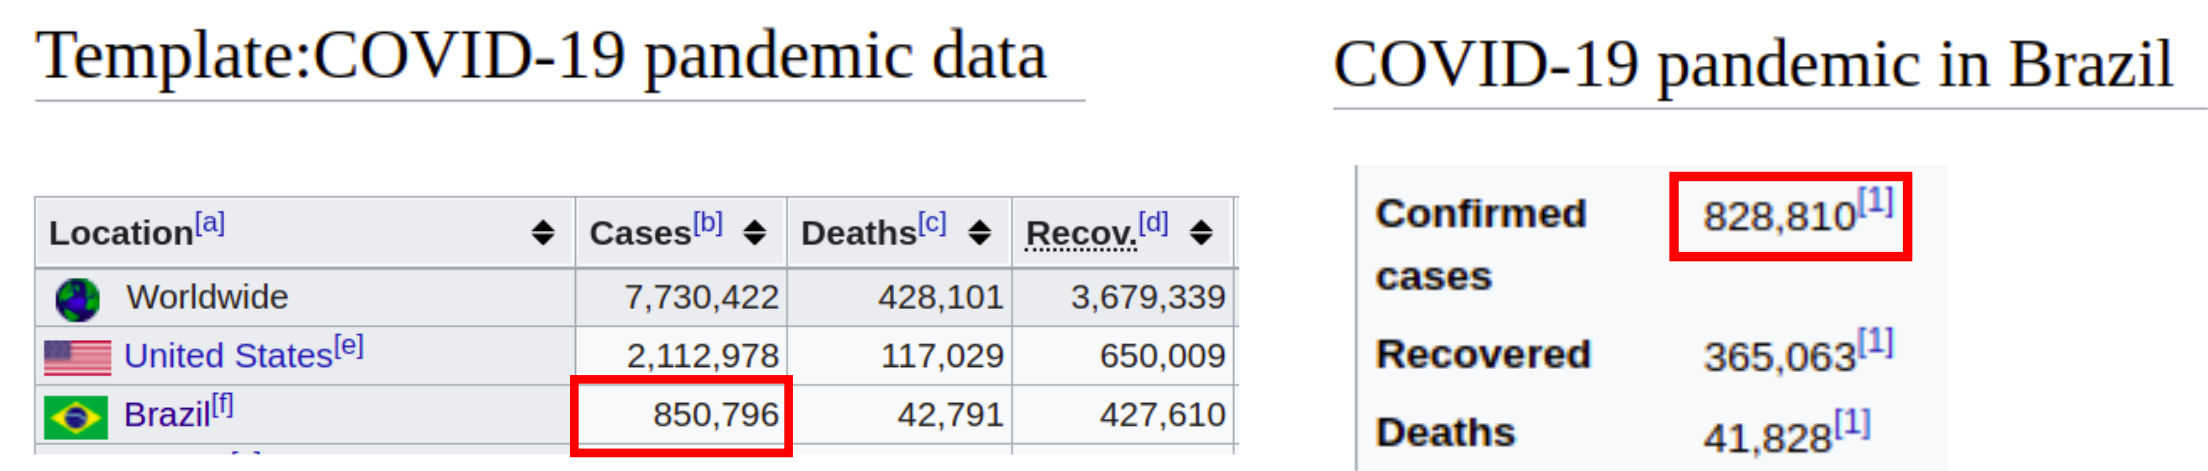
\includegraphics[scale=0.65]{fig/template_covid_19_brasil.png}
\end{figure}
and this is only one out of 309 different languages!
\end{frame}


\begin{frame}{Wikidata can be a hub to all Wikipedias}

\begin{itemize}
    \item Relationship to Wikipedia
    
    \begin{itemize}
        \item Moving structured data to Wikidata enables wide and reliable reuse
    \end{itemize}
\end{itemize}
\begin{figure}
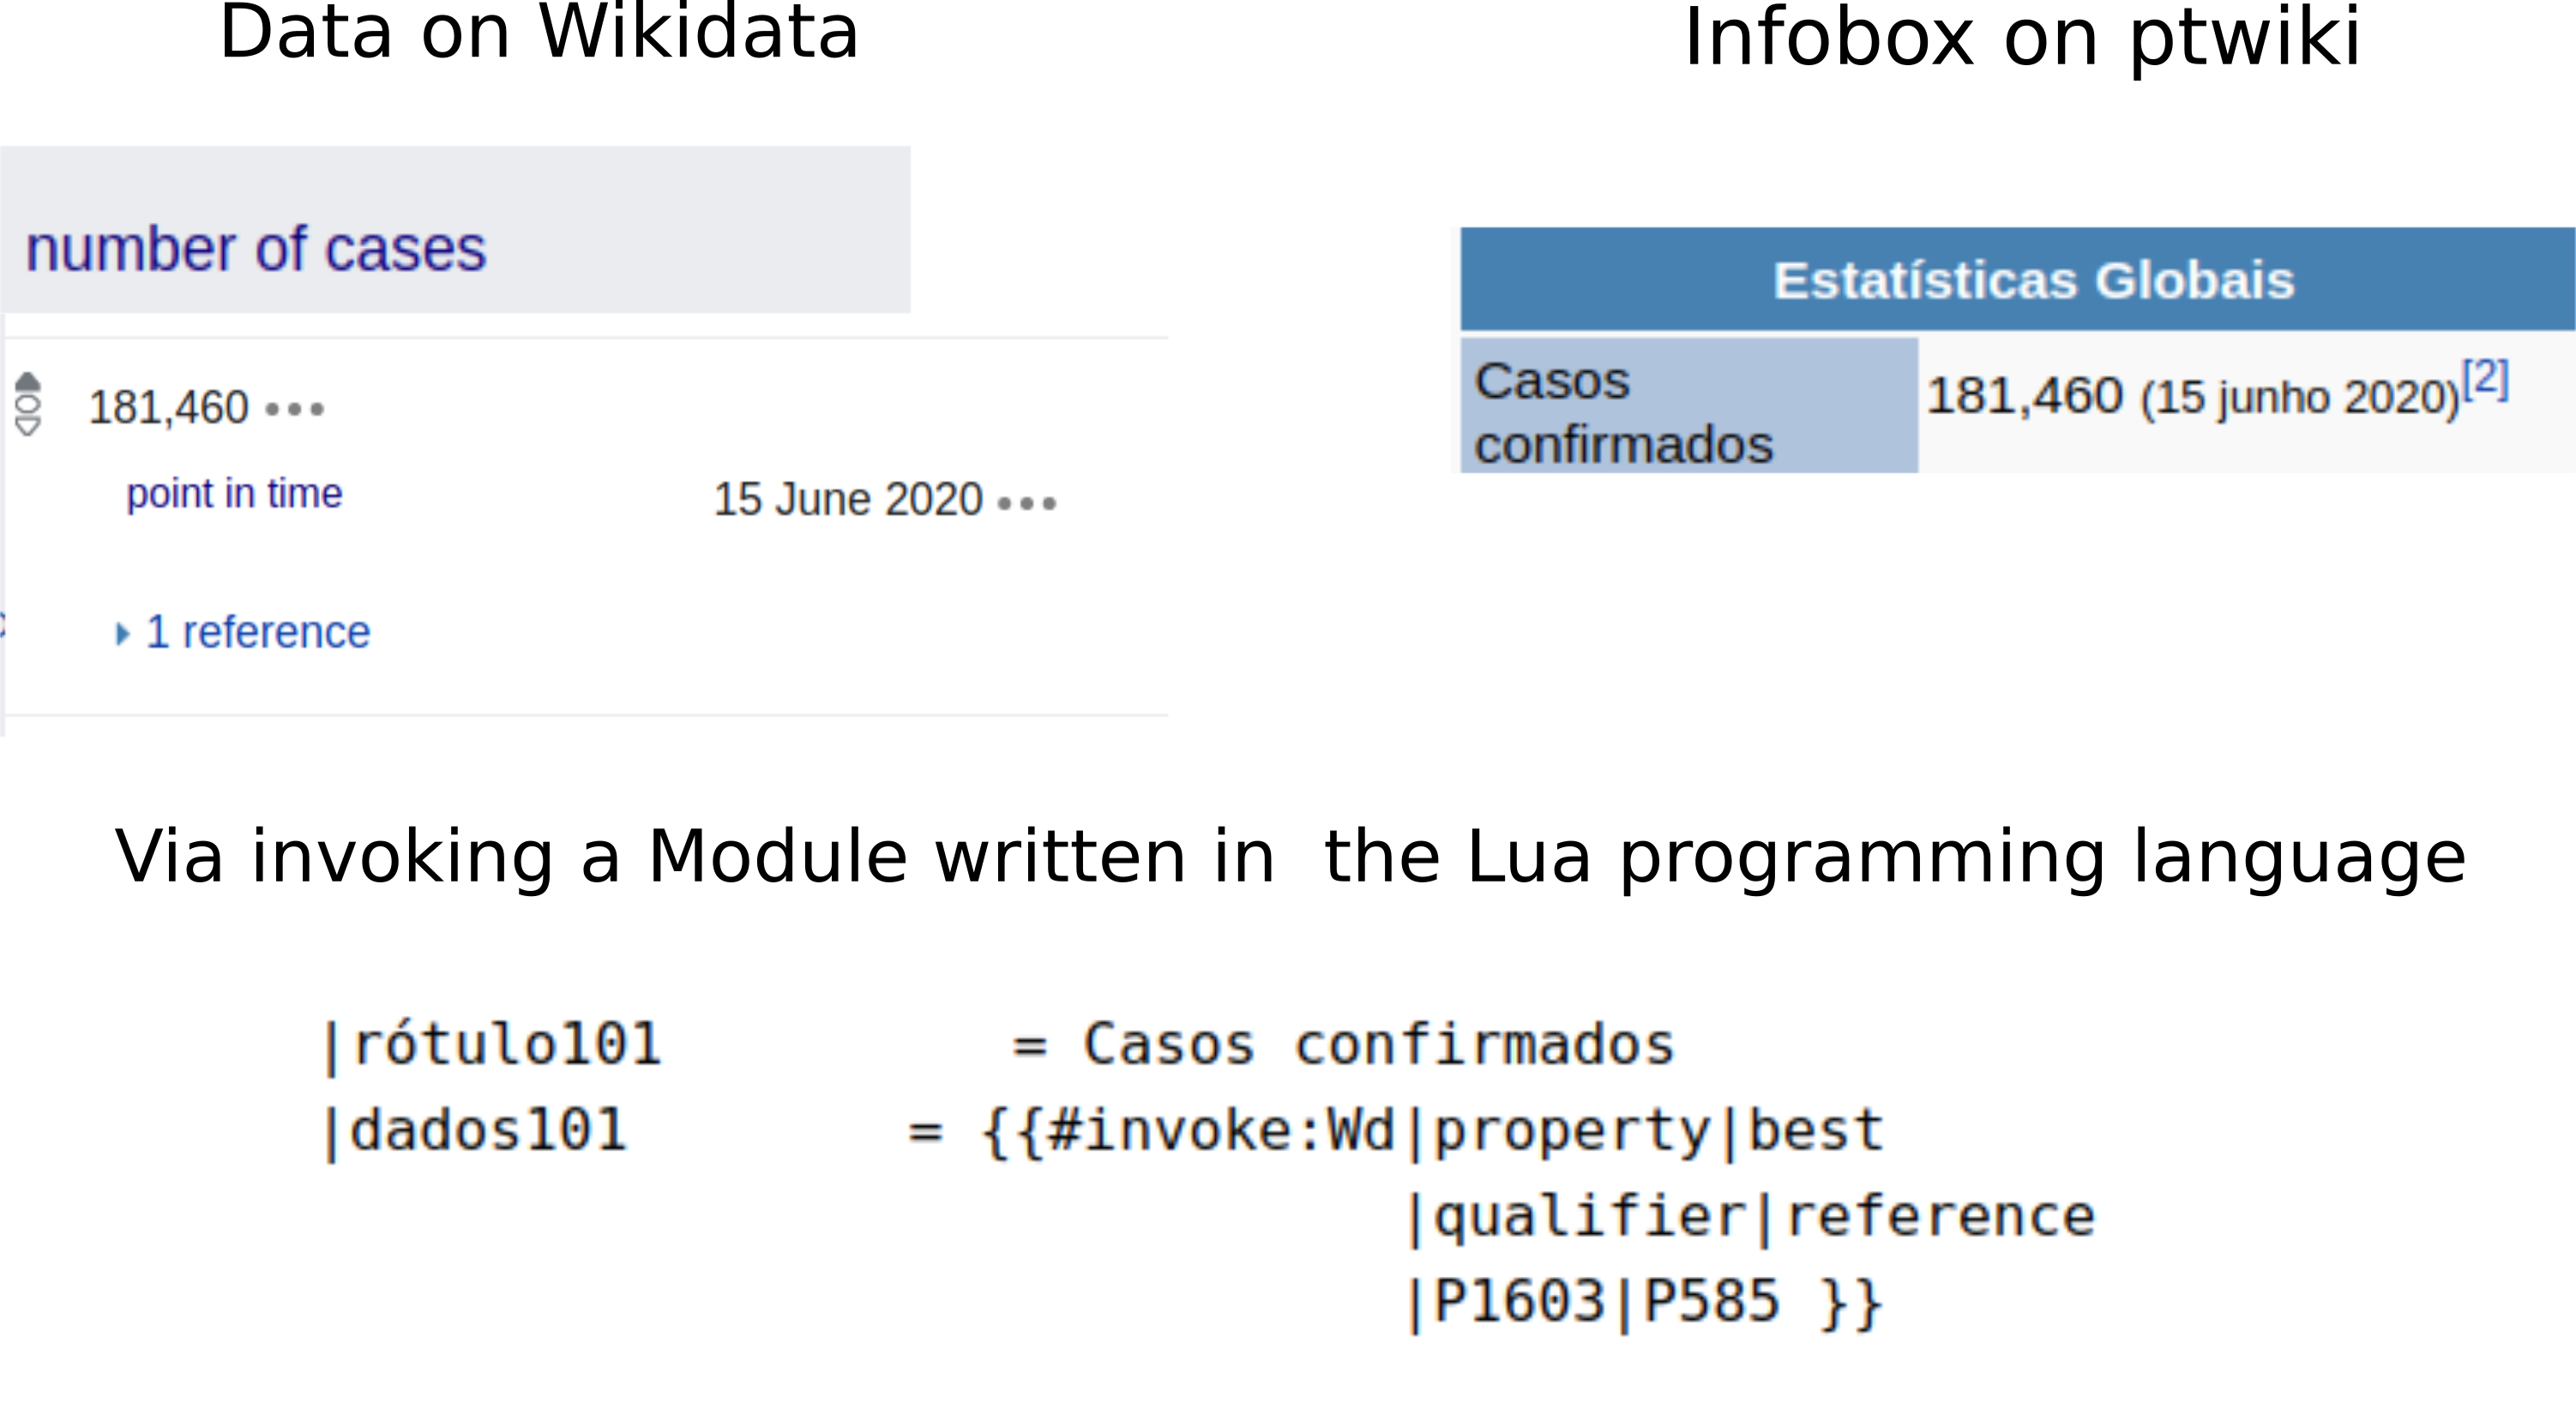
\includegraphics[scale=0.65]{fig/infobox_wikidata_on_pt_wiki.png}
\end{figure}

\end{frame}


\begin{frame}{Wikiproject COVID-19 came to accelarate this data structuring }

\begin{itemize}
    \item Wikidata is a relatively new project--> many things to improve!
    \item We united to organize open information about:
    
    \begin{itemize}
        \item Case, death and recovery counts
        \item Exploding scholarly literature on the disease
        \item Viral biology
        \item The policies and measures around the world
    \end{itemize}
\end{itemize}
\vskip 2cm

\url{wikidata.org/wiki/Wikidata:WikiProject_COVID-19}

\end{frame}


%%     \item Collaborative \& decentralized
%%    \item Challenging to coordinate and reach consensus


%% show examples 
\begin{frame}{Wikiproject COVID-19 - Standardization of data modelling}

\begin{itemize}
    \item Modeling number of cases (France) :
\end{itemize}

\begin{figure}
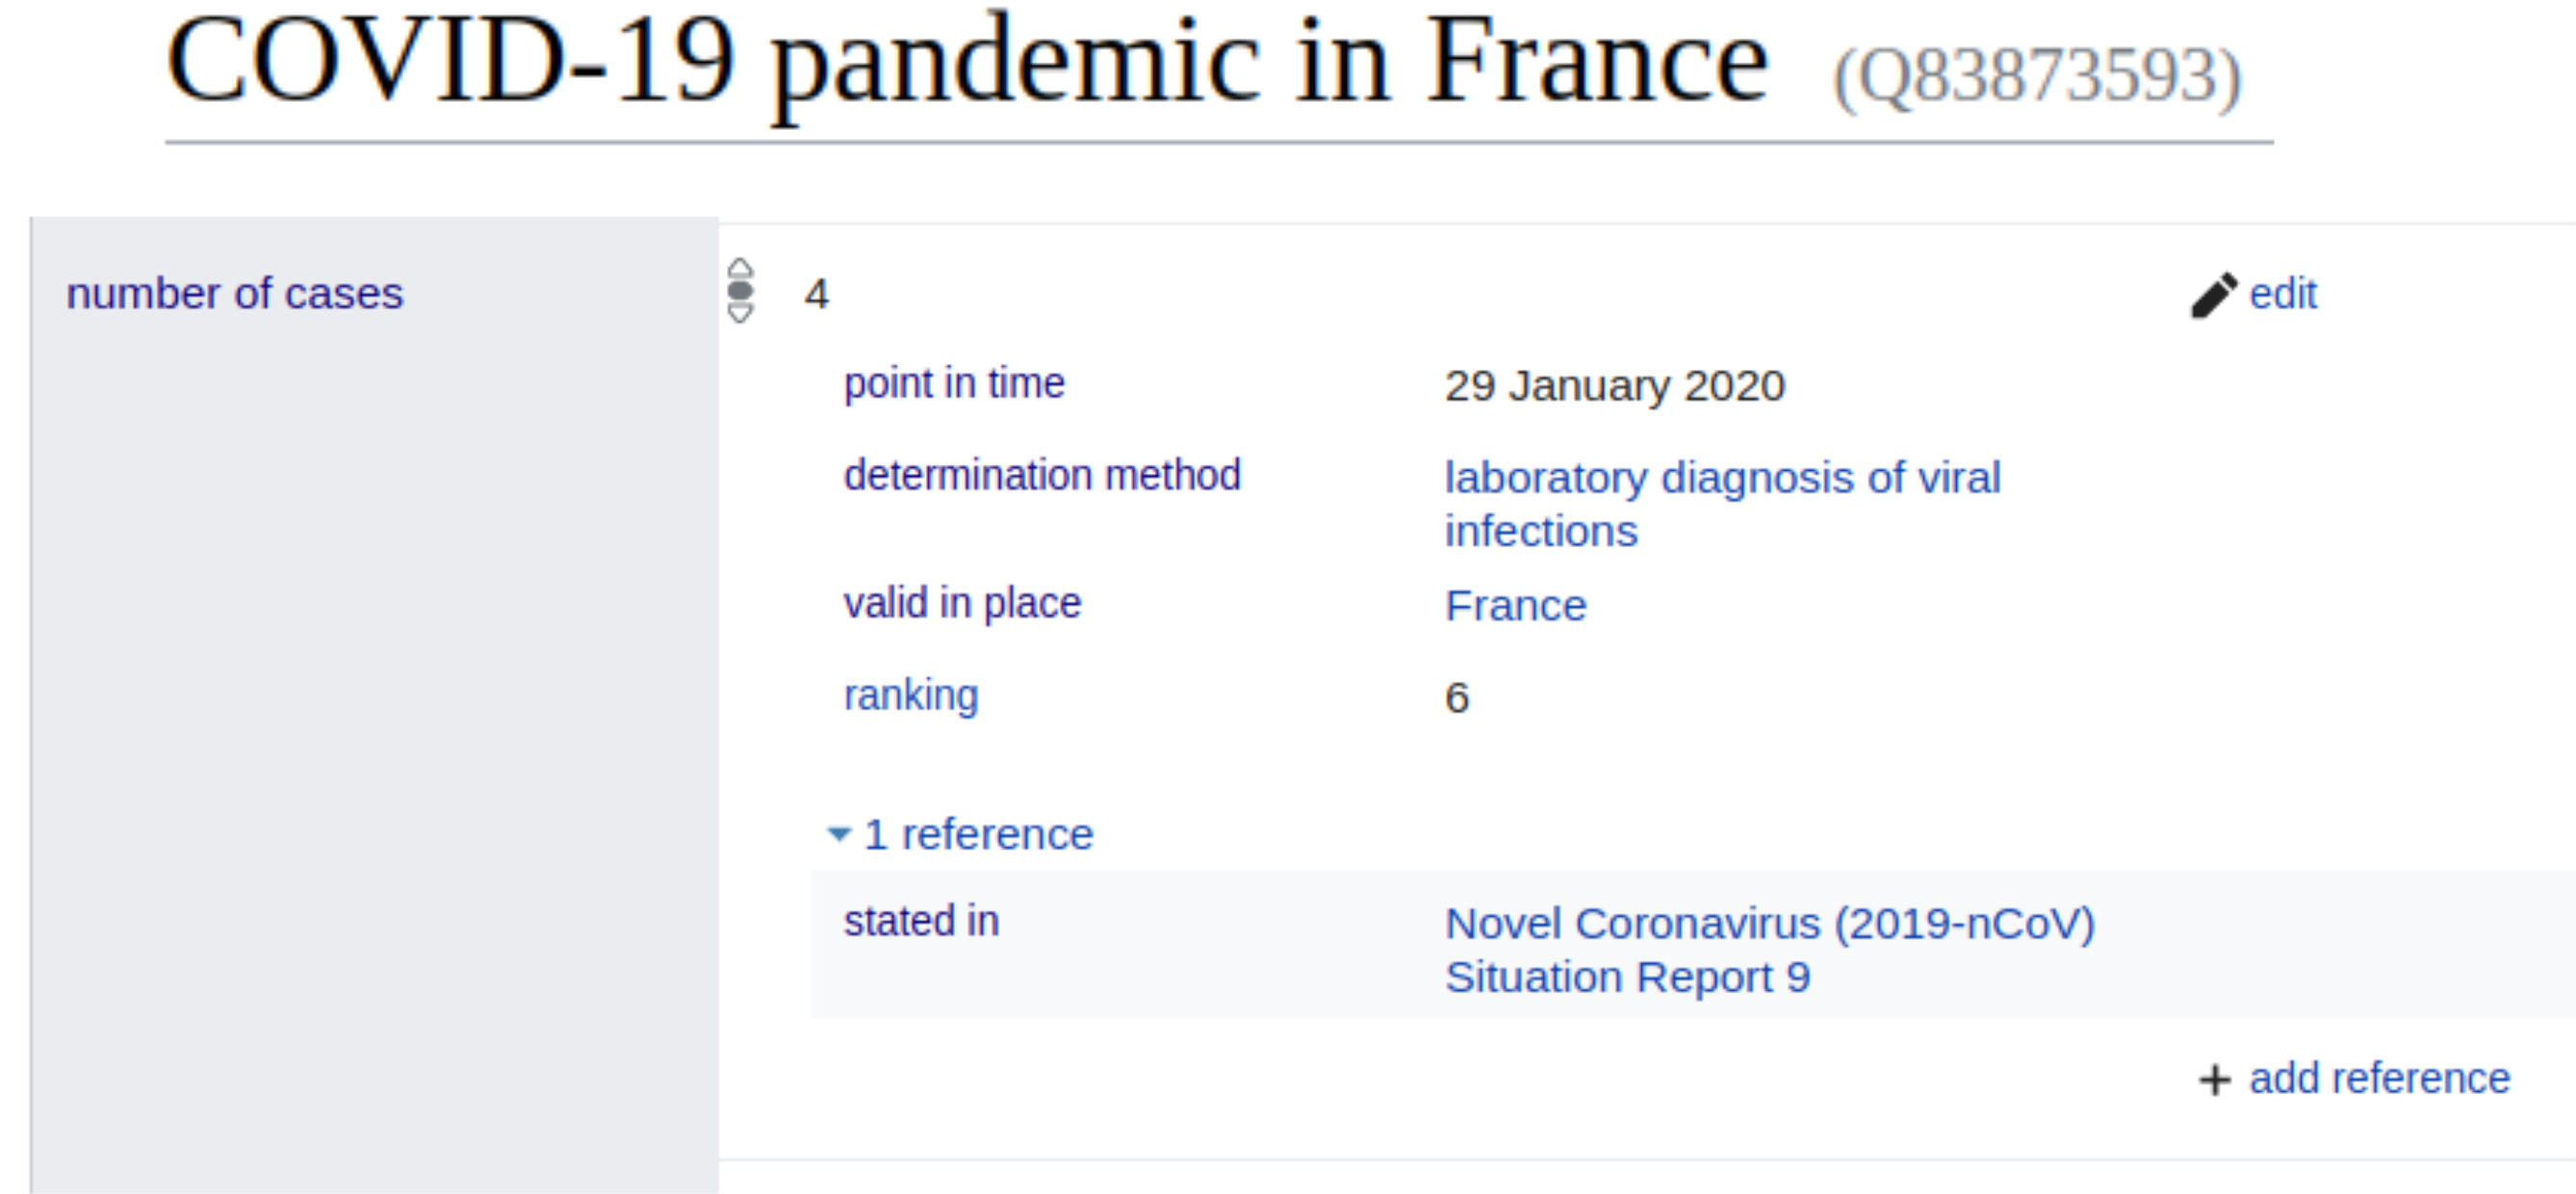
\includegraphics[scale=0.65]{fig/france_case_model.png}
\end{figure}

\end{frame}


\begin{frame}{Wikiproject COVID-19 - Standardization of data modelling}

\begin{itemize}
    \item Modeling number of cases (Sweden) :
\end{itemize}

\begin{figure}
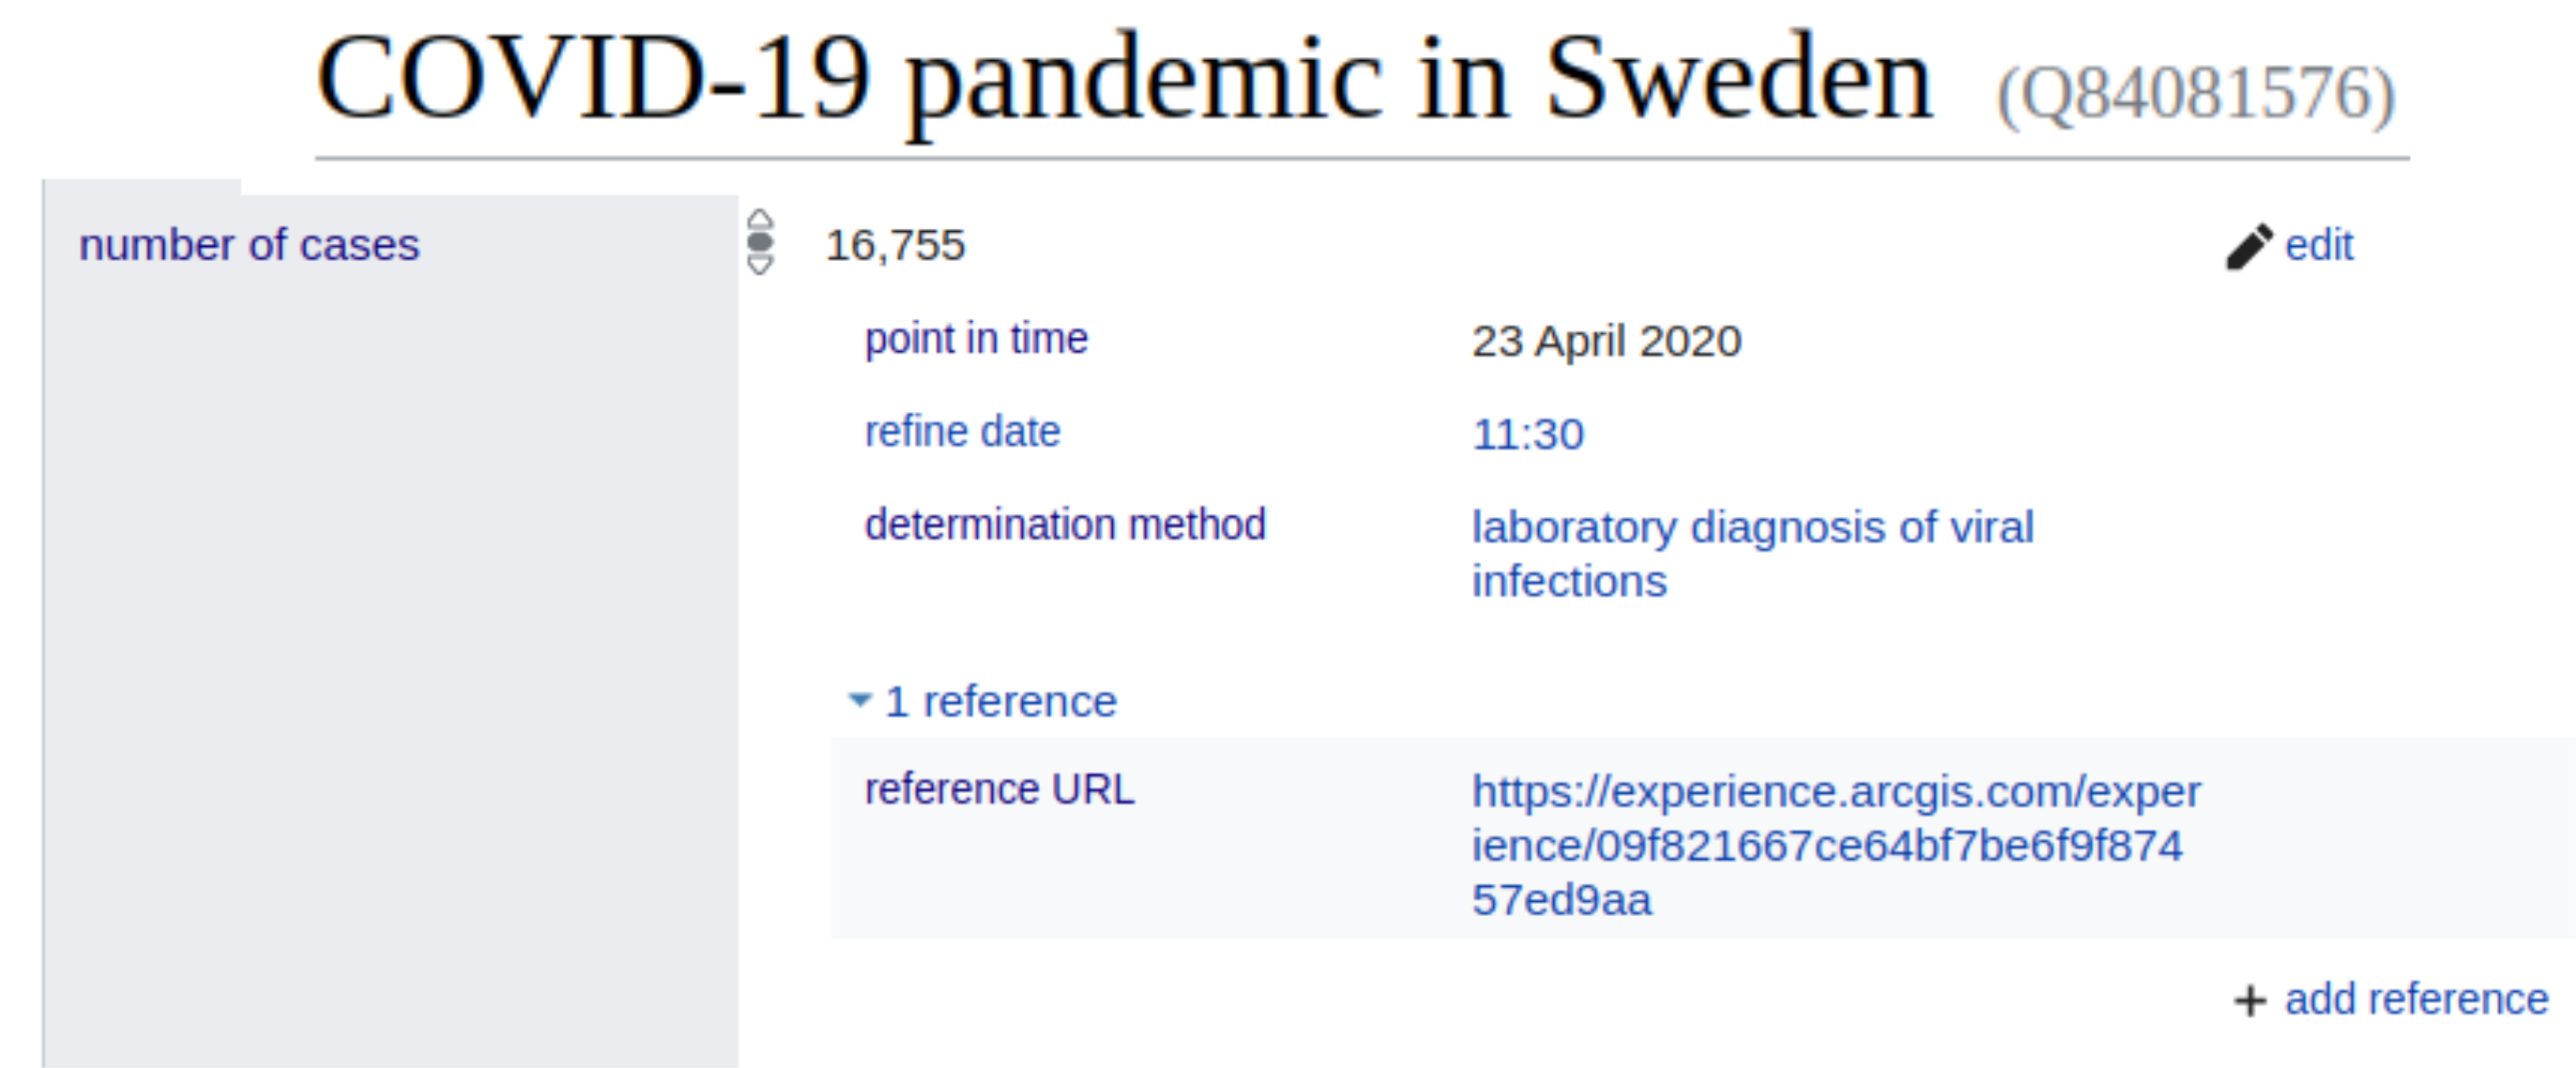
\includegraphics[scale=0.65]{fig/sweden_case_model.png}
\end{figure}

\end{frame}


\begin{frame}{Finding consensus in a community}
\begin{itemize}
    \item People brought experiences and opinions to WikiProject Talk Pages
\end{itemize}

\begin{figure}
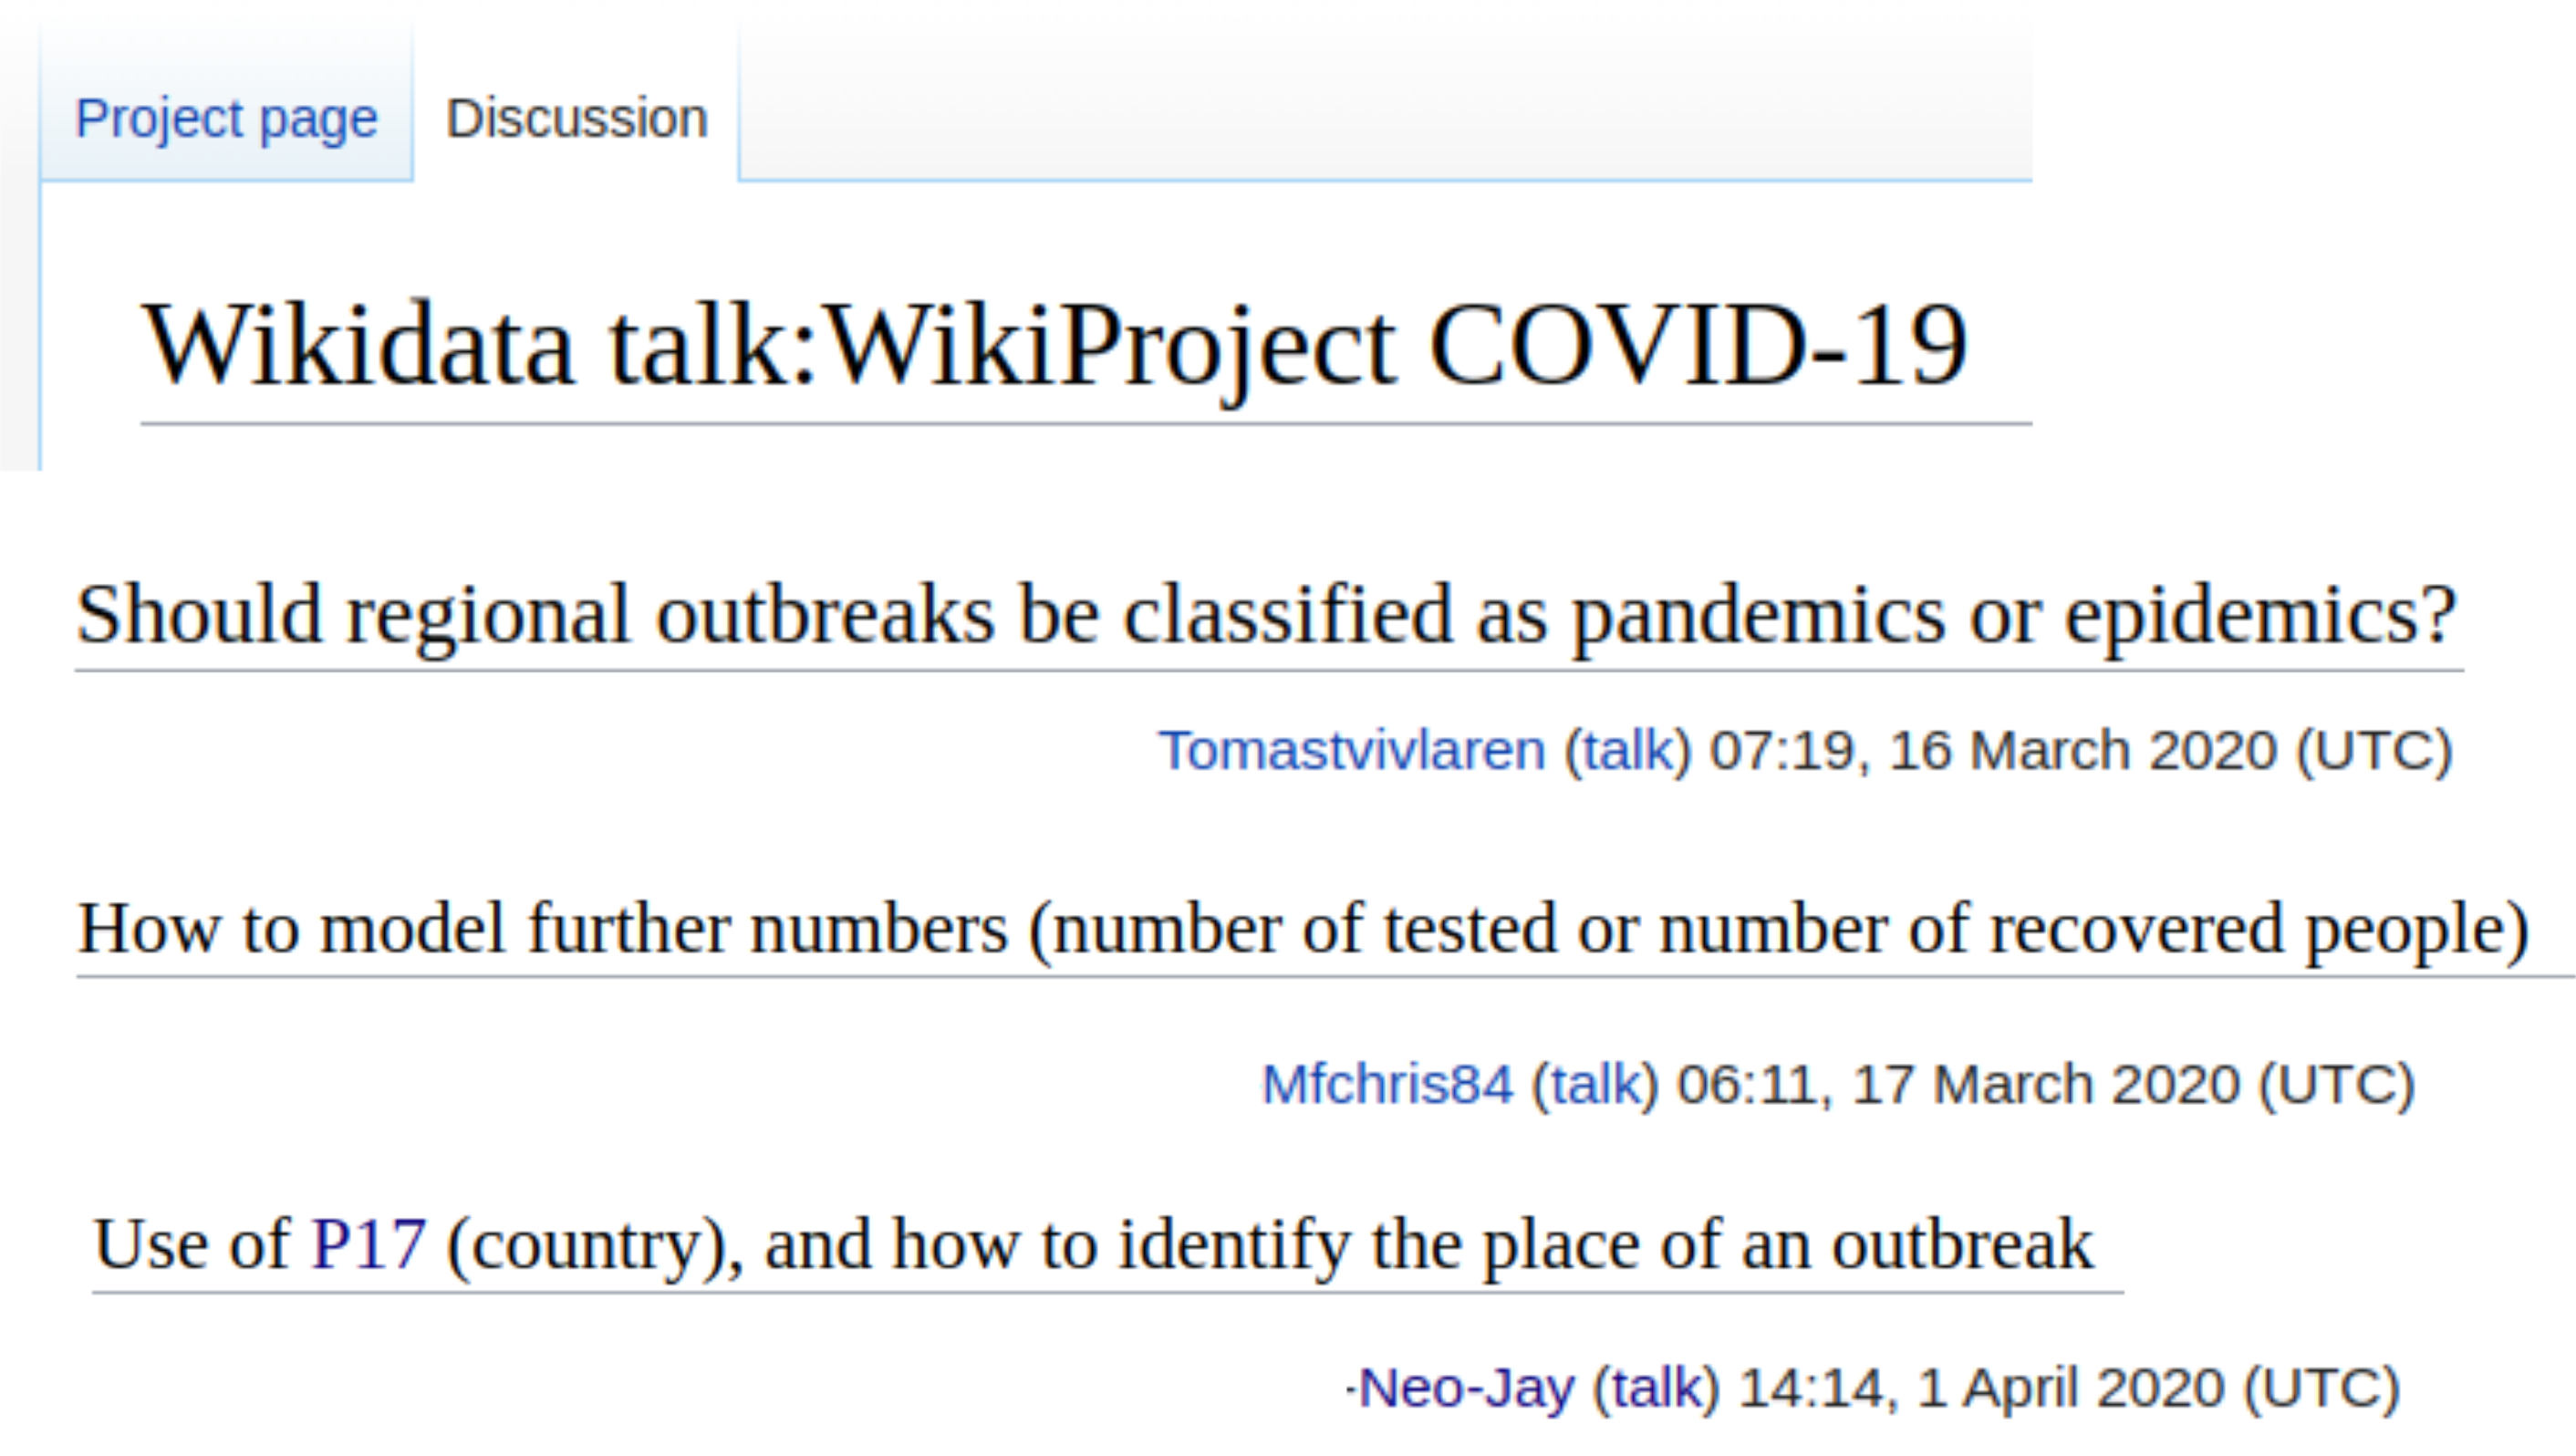
\includegraphics[scale=0.65]{fig/discussion_headers.png}
\end{figure}

\end{frame}


\begin{frame}{Finding consensus in a community}
\begin{itemize}
    \item We had good, respectful discussions 
\end{itemize}

\begin{figure}
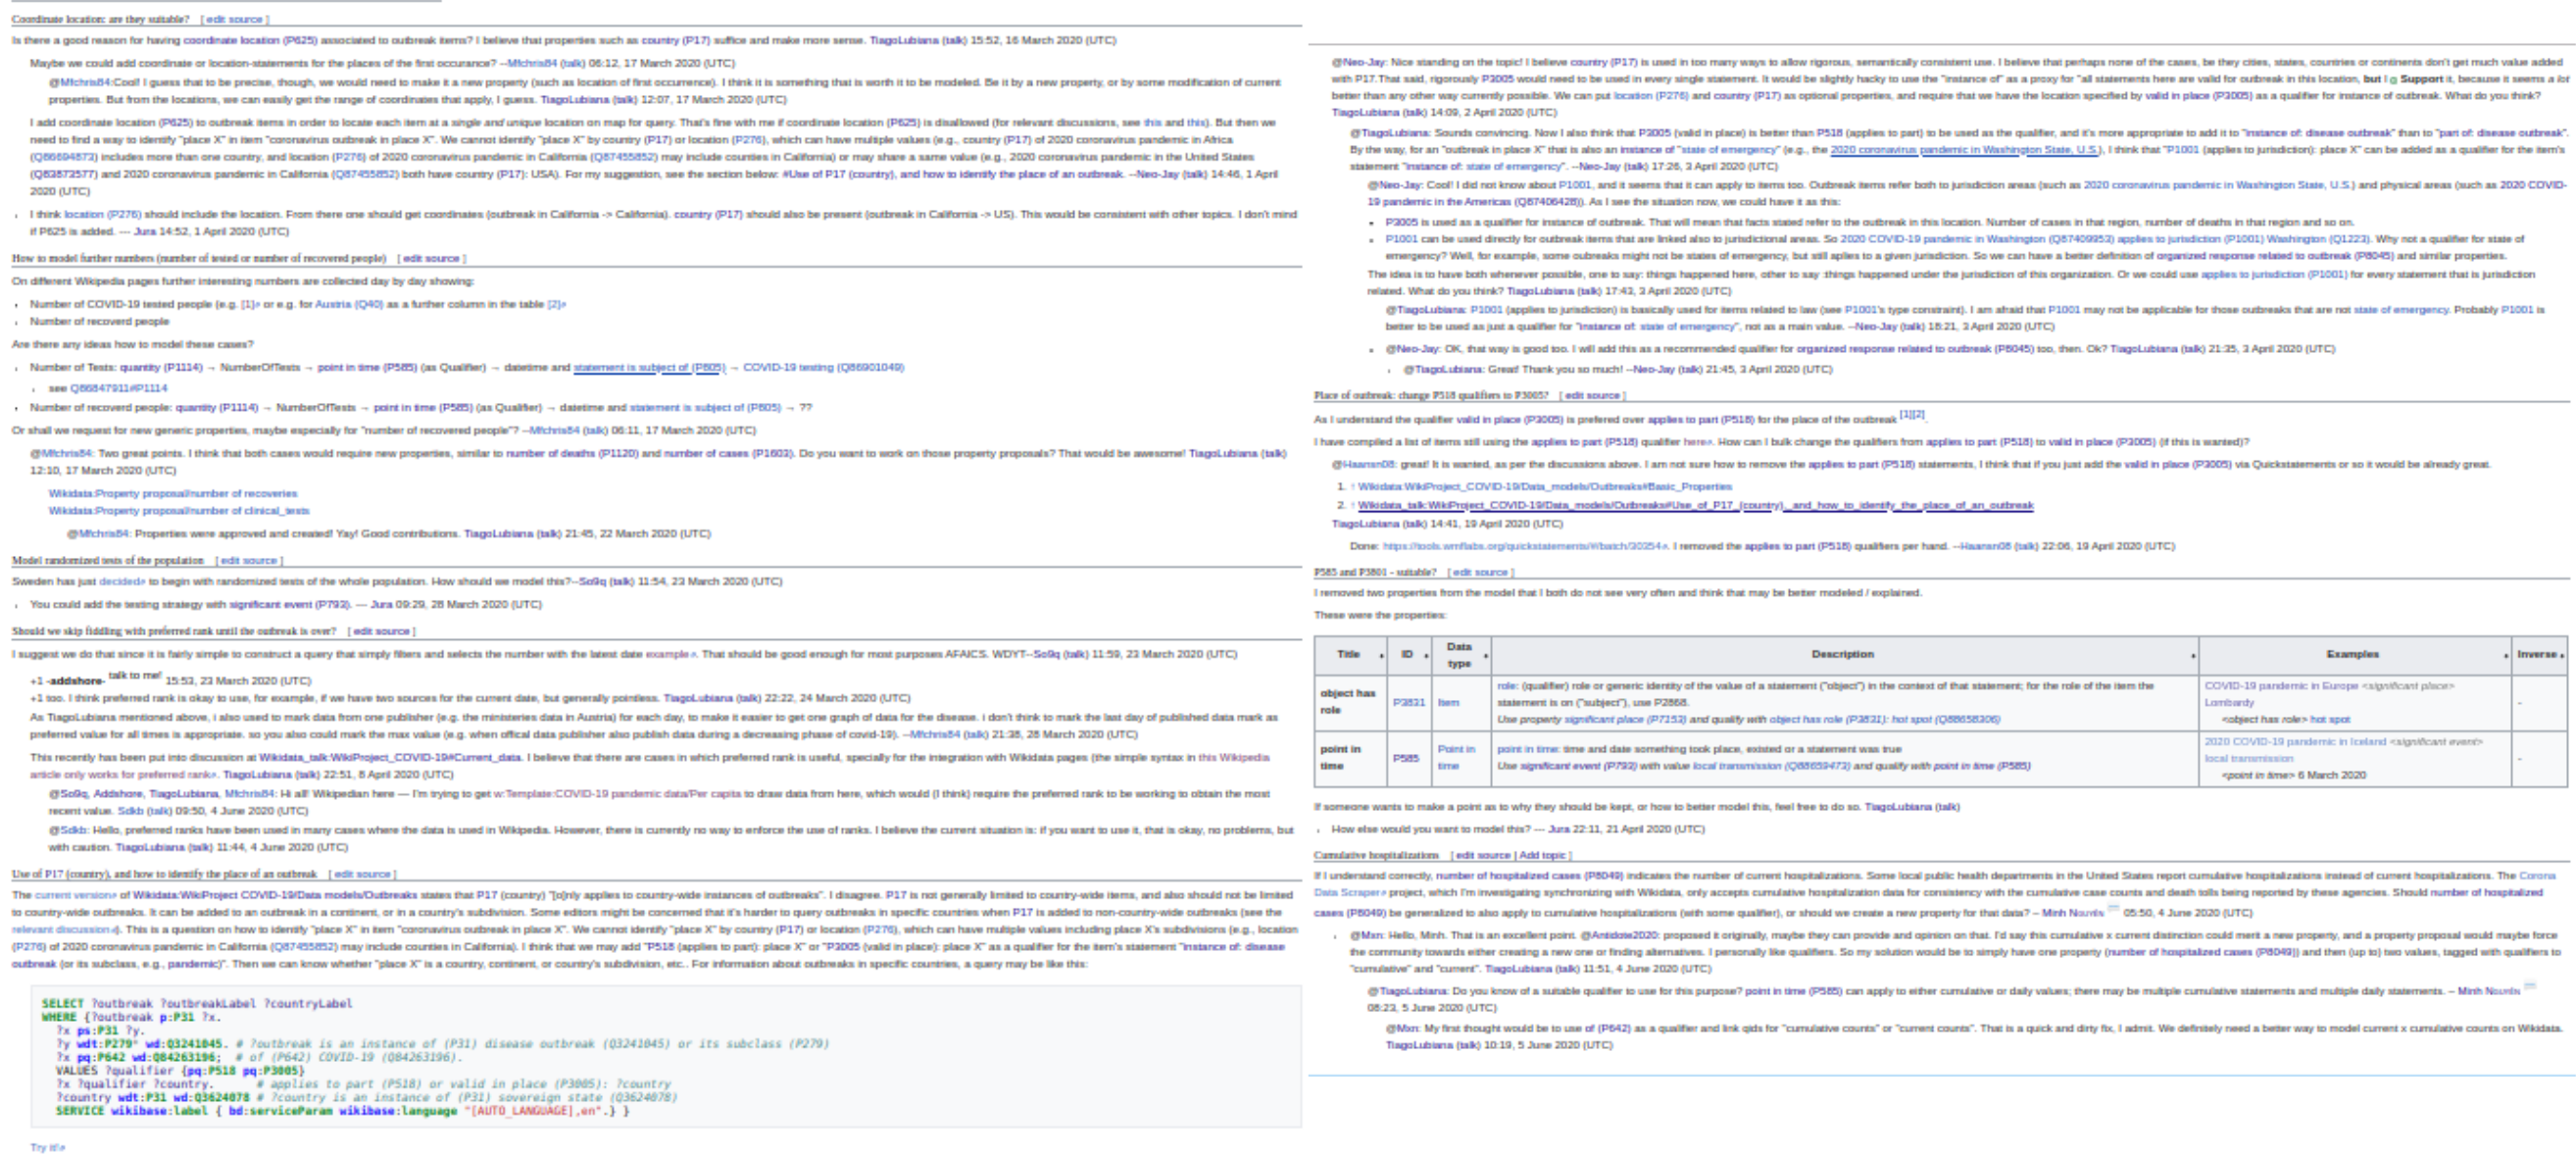
\includegraphics[scale=0.65]{fig/discussions_text.png}
\end{figure}

\end{frame}


\begin{frame}{Finding consensus in a community}
\begin{itemize}
    \item The results of the discussions were transferred to a "guide page"
    \item A non-mandatory guide for how items should be represented
    
\end{itemize}

\begin{figure}
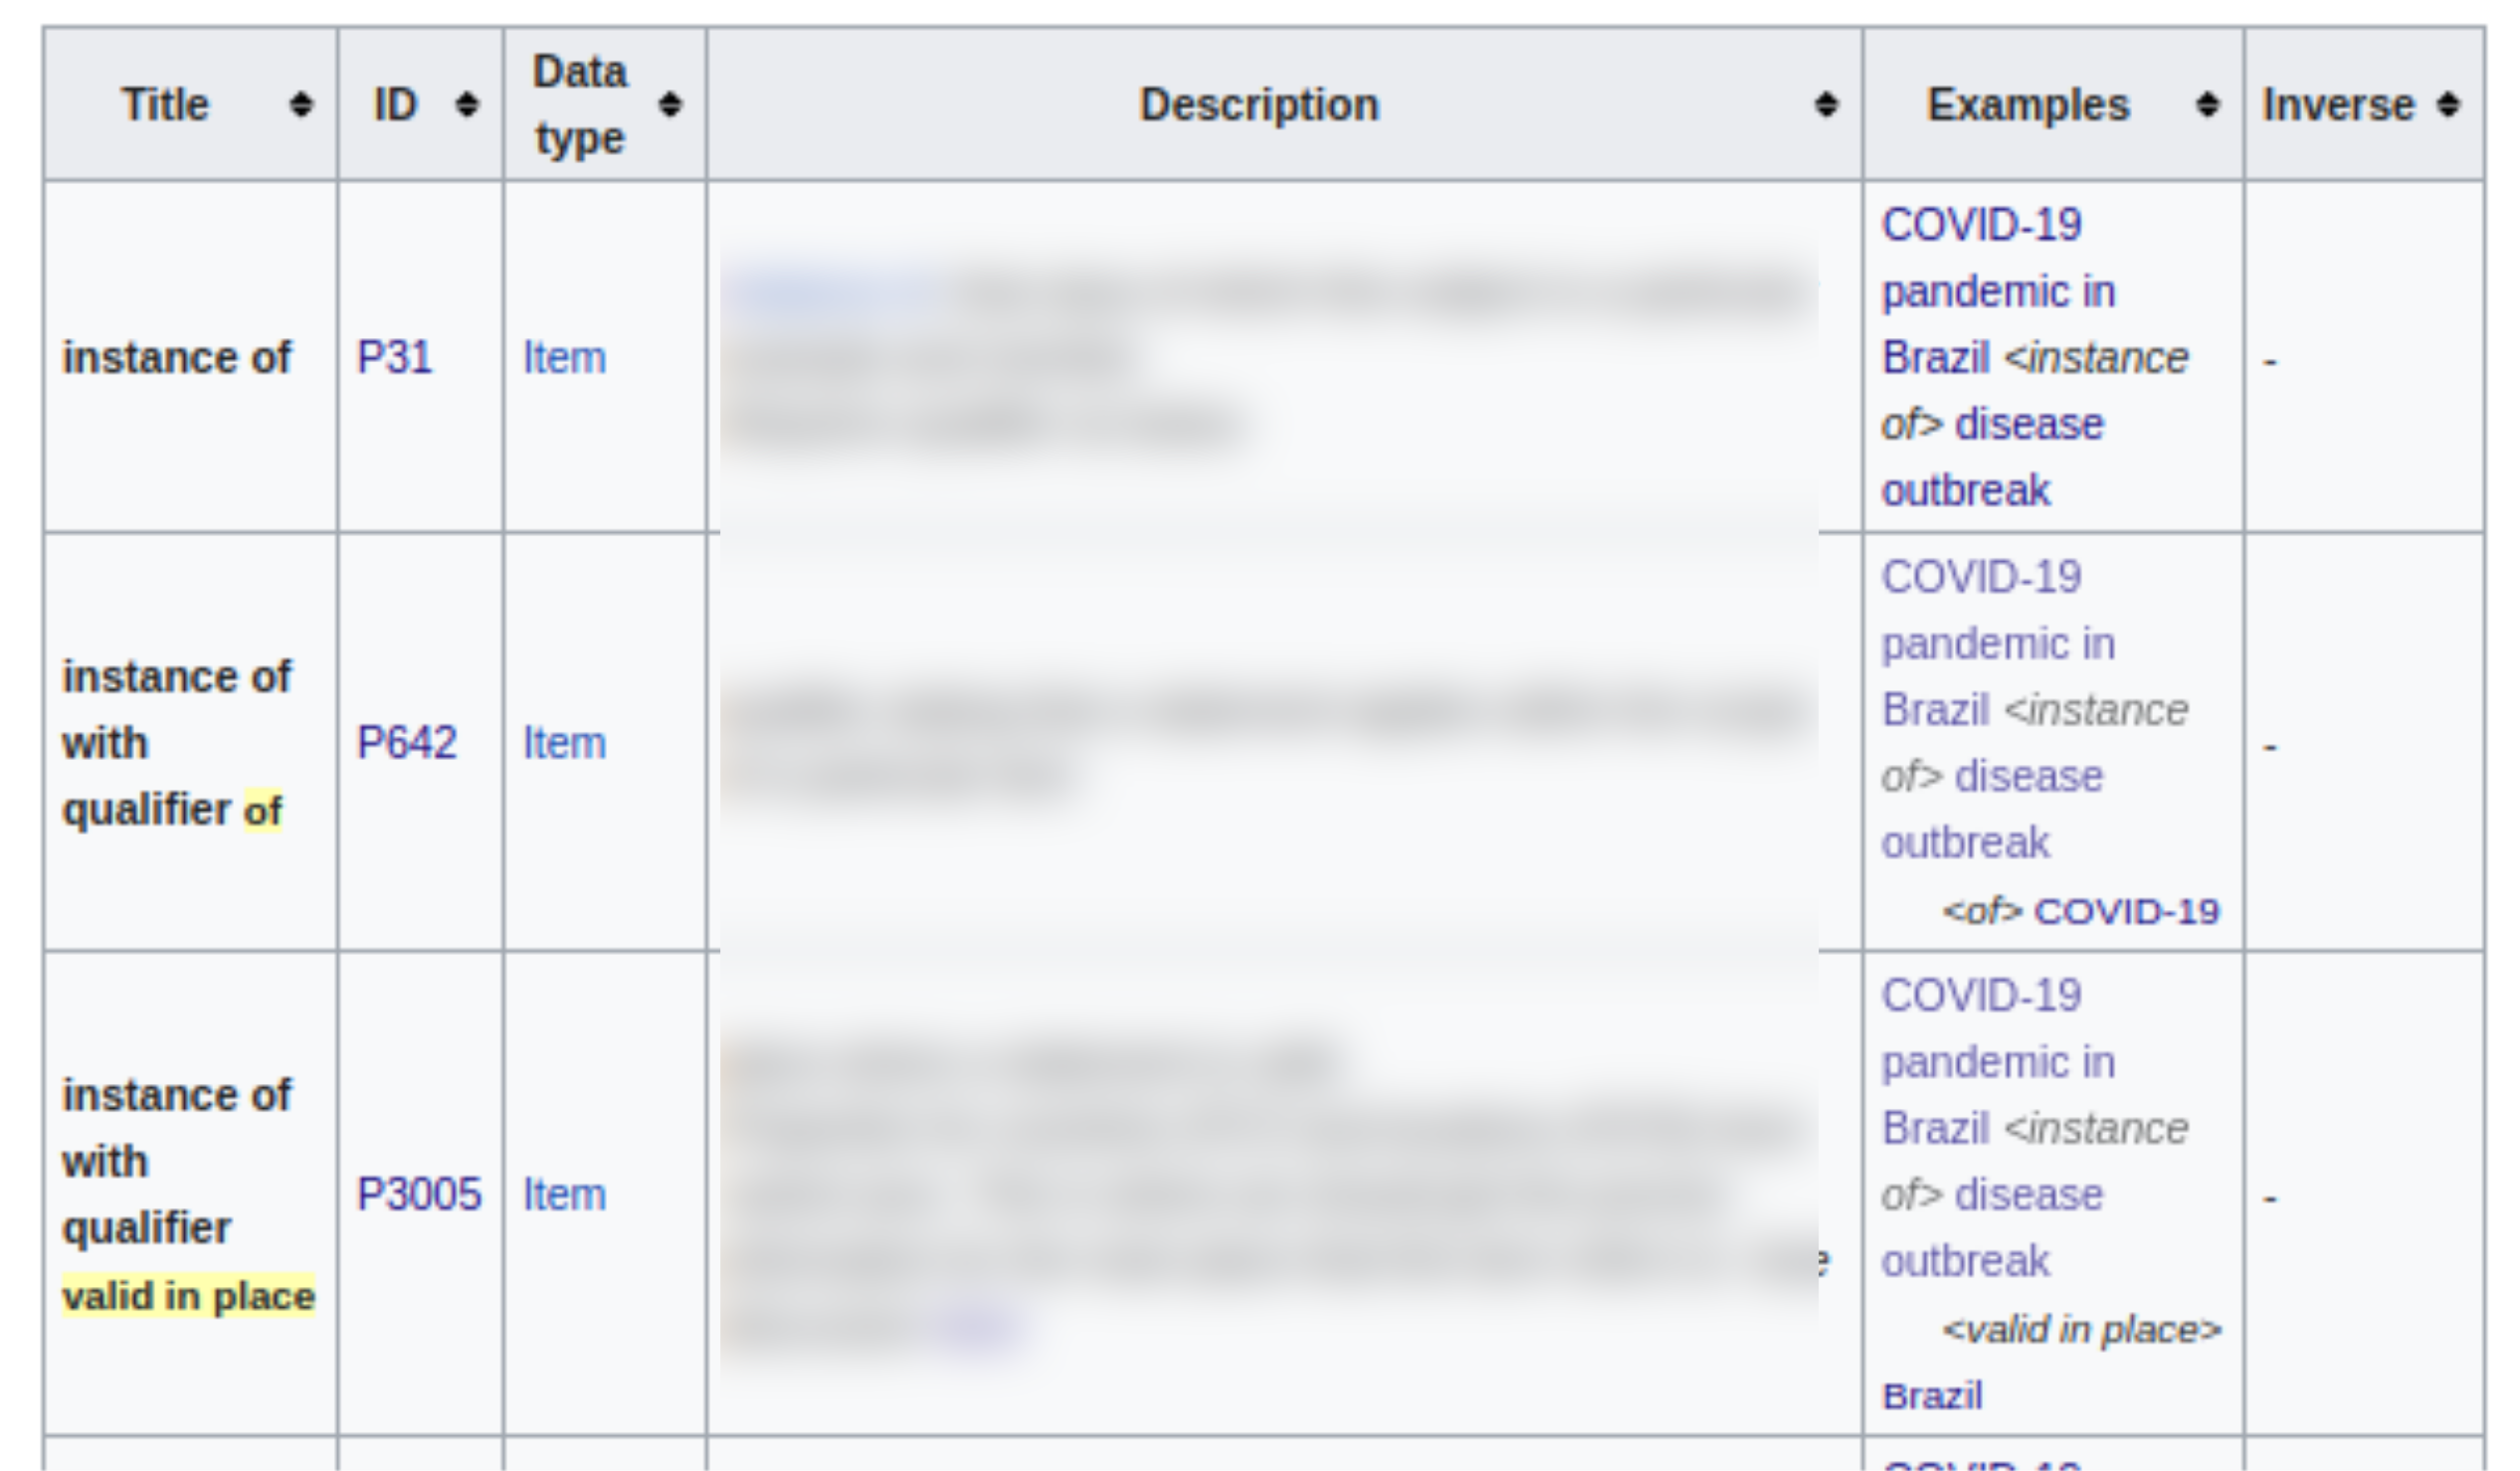
\includegraphics[scale=0.65]{fig/outbreak_datamodel_table.png}
\end{figure}
\end{frame}


\begin{frame}{Finding consensus in a community}
\begin{itemize}
    \item And recommendations guide the database uploads
\end{itemize}

\begin{figure}

\includegraphics[scale=0.65]{fig/model_evolution.png}
\end{figure}

\end{frame}

% Data models are innocent until proven otherwise.

\begin{frame}{Finding consensus in a community}
\begin{itemize}
    \item These data models are eventually represented in more rigorous format: Shape Expression (ShEx)
    \item Example for hospitals:
\end{itemize}
\begin{figure}
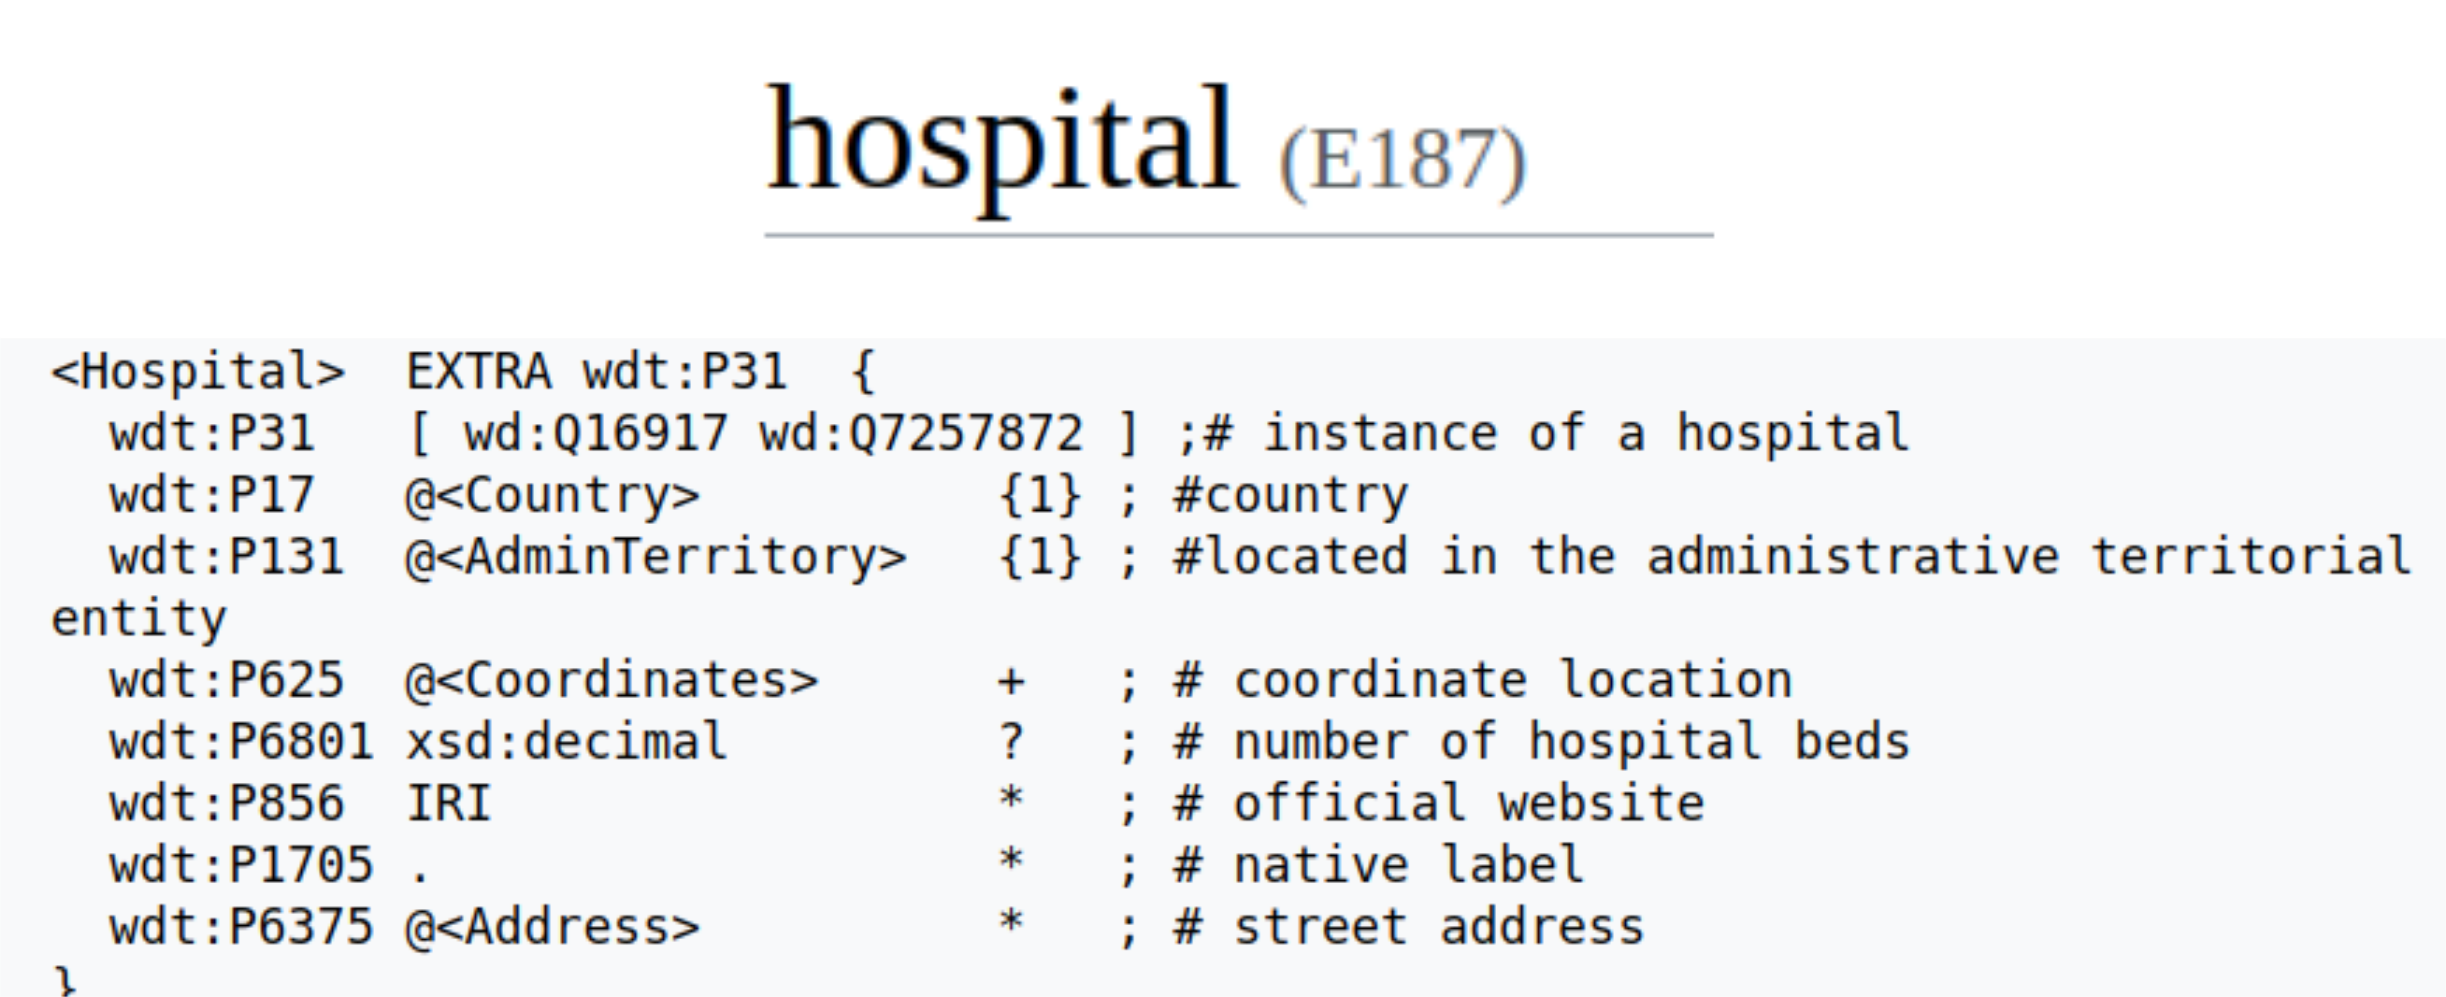
\includegraphics[scale=0.65]{fig/shex_hospitals.png}
\end{figure}
\end{frame}

%Mention validation 



\begin{frame}{Properly structured data can be used for visualization}
\begin{itemize}
    \item Wikidata Queries using the SPARQL query system 
    \item We can visualize, for example, individuals that died from COVID-19
\end{itemize}
\begin{figure}
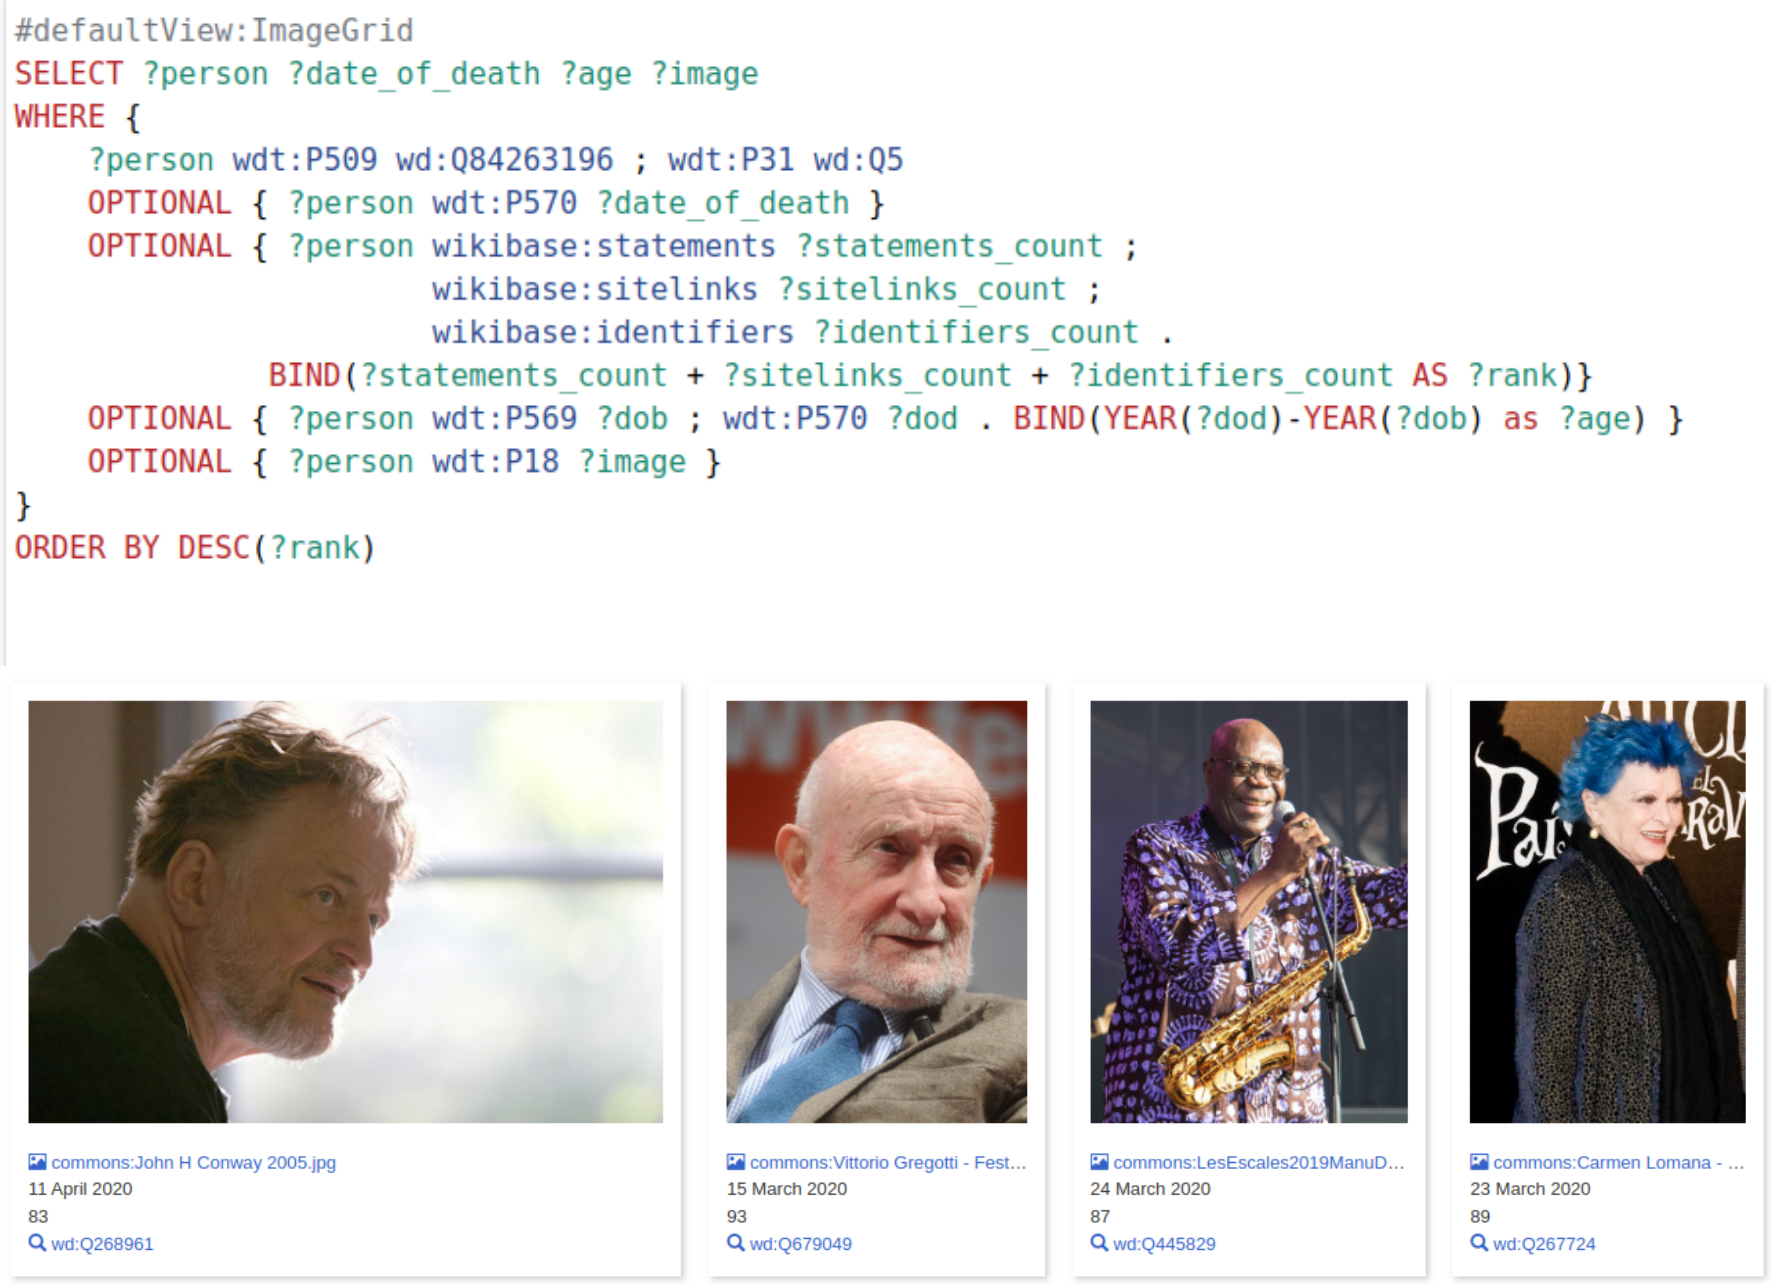
\includegraphics[scale=0.65]{fig/covid19_deaths.png}
\end{figure}
\end{frame}

\begin{frame}{Next steps of the Wikiproject Covid19}
\begin{itemize}
    \item Parse and integrate external databases
\end{itemize}
\begin{figure}
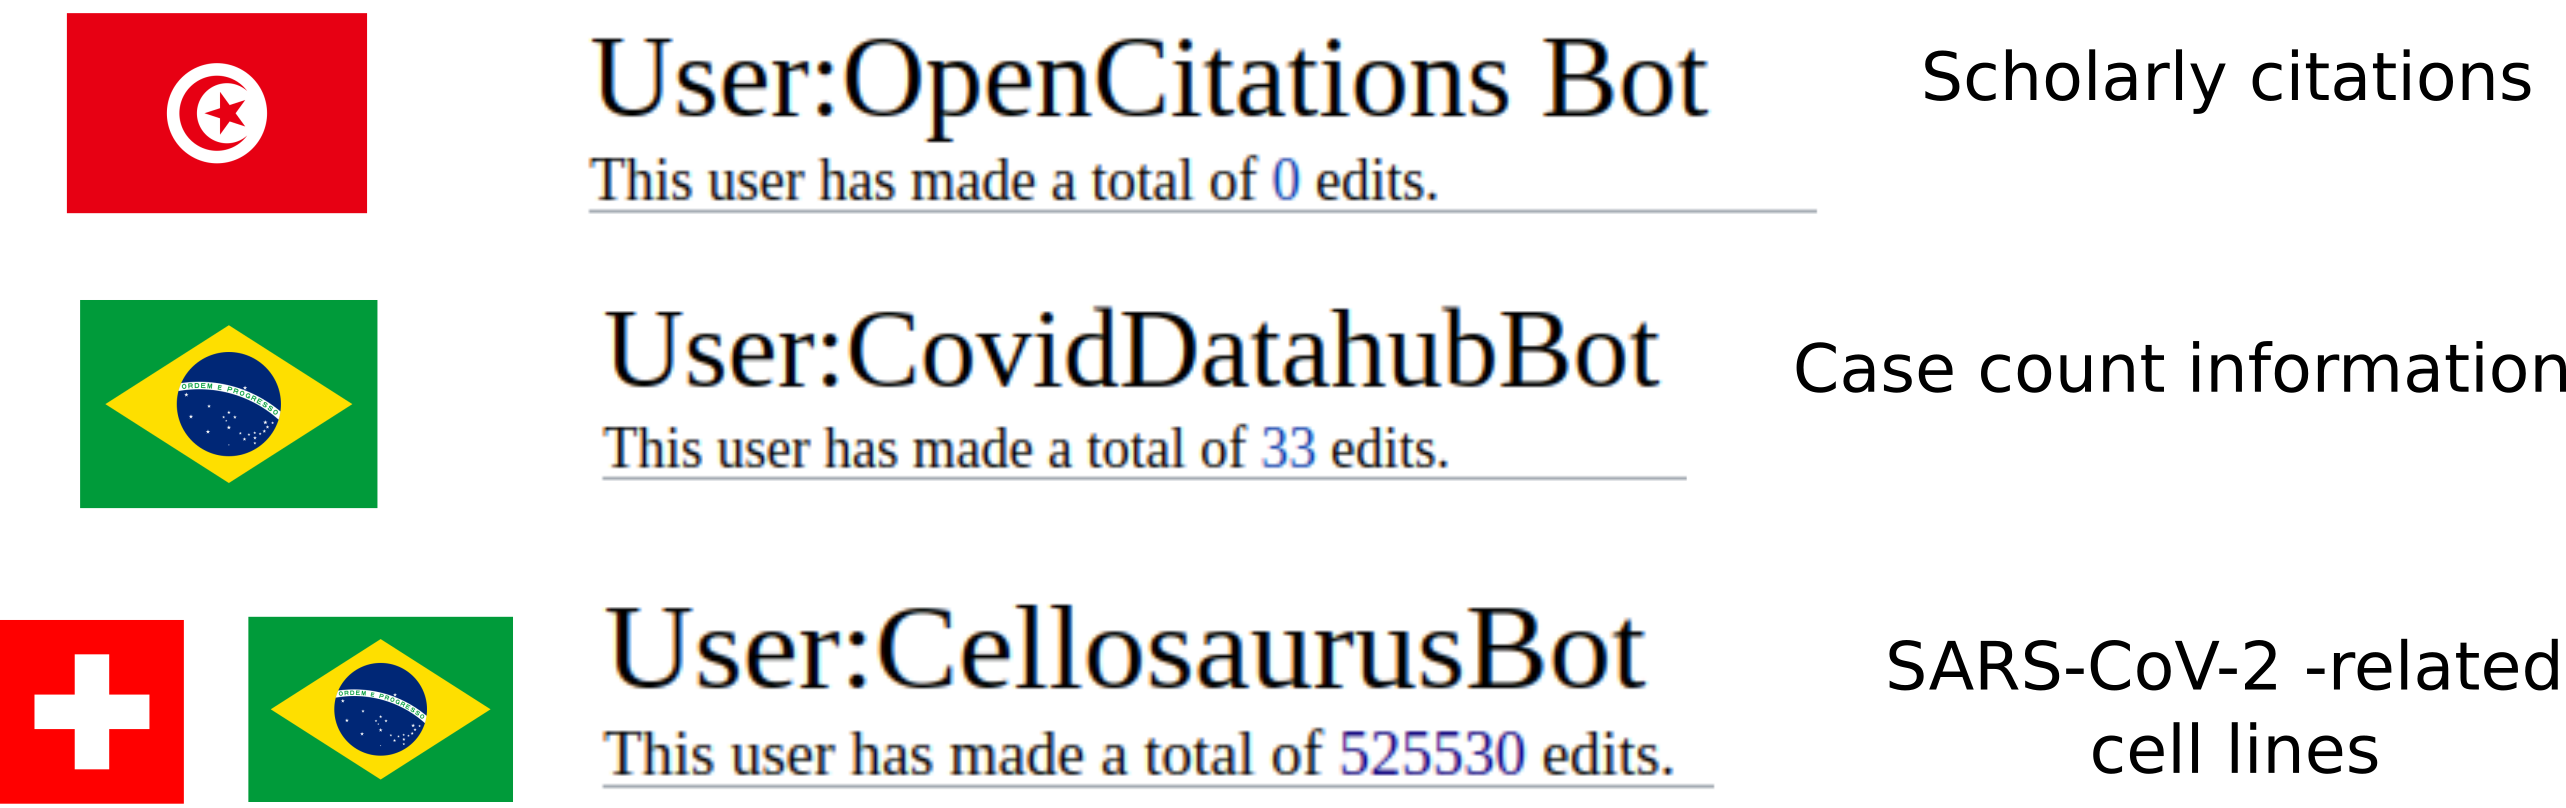
\includegraphics[scale=0.65]{fig/wikidata_covid_19_bots.png}
\end{figure}
\end{frame}

\begin{frame}{Next steps of the Wikiproject Covid19}
\begin{itemize}
    \item Improve the quality control of items of interest (maybe via ShEx?) 
\end{itemize}
\begin{figure}
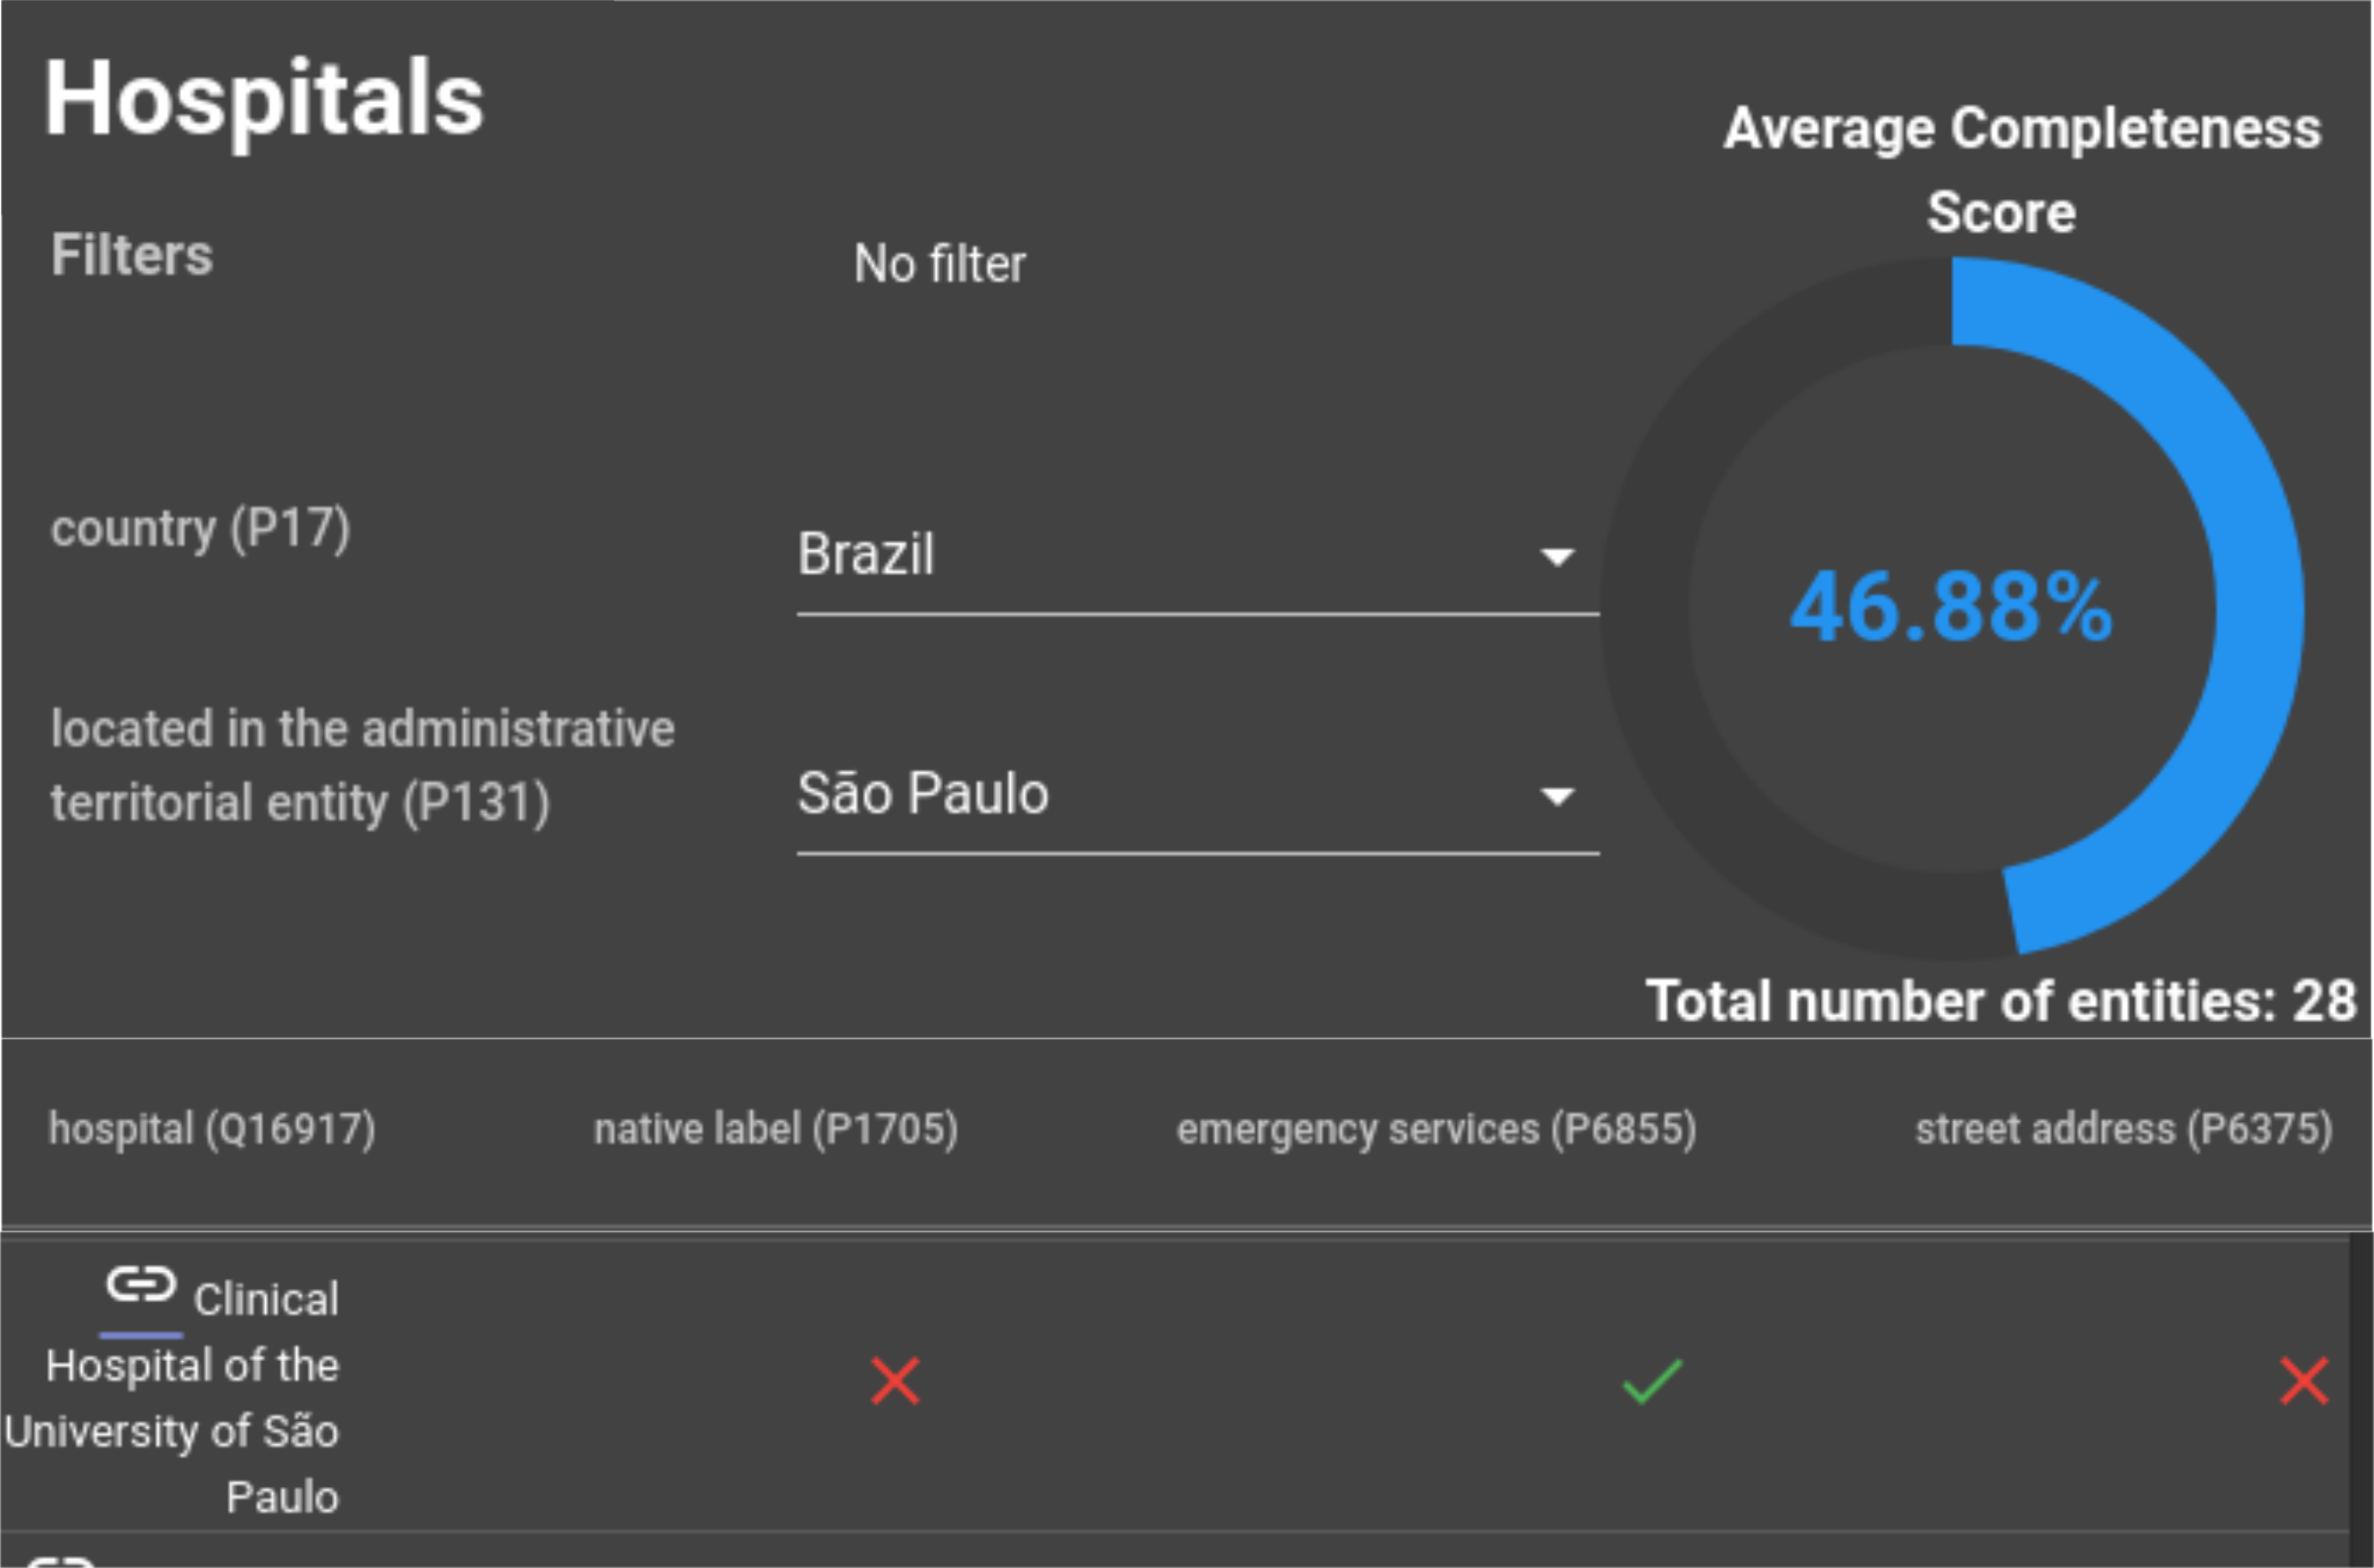
\includegraphics[scale=0.65]{fig/validation.png}
\end{figure}
\end{frame}

\begin{frame}{Next steps of the Wikiproject Covid19}
\begin{itemize}
    \item Spread the word! Anyone can contribute to and benefit from Wikidata. 
\end{itemize}
\begin{figure}

\includegraphics[scale=0.65]{fig/dcmi.png}
\end{figure}
\end{frame}




\begin{frame}
  \titlepage
\end{frame}
{
\setbeamercolor{background canvas}{bg=}

\includepdf[pages=1]{fig/last_slide.pdf}
}


\end{document}